\documentclass[12pt]{article}
\usepackage{amsmath}
\usepackage{times}
\usepackage{graphicx}
\graphicspath{{../}}
\usepackage{color}
\usepackage{multirow}
\usepackage{placeins}
\usepackage{mathptmx} % Times-like text + math
\usepackage[T1]{fontenc}
\usepackage{hyperref}
\usepackage{makecell}
\usepackage{booktabs}
\usepackage{tabularx}
\usepackage{amsmath, amssymb}
\usepackage{array}

%%%
\usepackage{tabularx,booktabs}
\usepackage{ragged2e}
\newcolumntype{Y}{>{\RaggedRight\arraybackslash}X}

\usepackage{natbib}
\bibliographystyle{apalike}


\usepackage{setspace}
\setstretch{1.05}

\usepackage{microtype}
\setlength{\emergencystretch}{2em}

\usepackage{graphicx}
%\usepackage[authoryear]{natbib}
%
\usepackage{bbm}
\usepackage{latexsym}
%\DeclareGraphicsExtensions{.eps,.png}

%%% margins 
\textheight 23.4cm
\textwidth 14.65cm
\oddsidemargin 0.375in
\evensidemargin 0.375in
\topmargin  -0.55in
%
\renewcommand{\baselinestretch}{1.05}
%
\interfootnotelinepenalty=10000
%
\renewcommand{\thesubsubsection}{\arabic{section}.\arabic{subsubsection}}
\newcommand{\myparagraph}[1]{\ \\{\em #1}.\ \ }
\newcommand{\citealtt}[1]{\citeauthor{#1},\citeyear{#1}}
\newcommand{\myycite}[1]{\citep{#1}}

% Different font in captions
\newcommand{\captionfonts}{\normalsize}

\makeatletter  
\long\def\@makecaption#1#2{%
  \vskip\abovecaptionskip
  \sbox\@tempboxa{{\captionfonts #1: #2}}%
  \ifdim \wd\@tempboxa >\hsize
    {\captionfonts #1: #2\par}
  \else
    \hbox to\hsize{\hfil\box\@tempboxa\hfil}%
  \fi
  \vskip\belowcaptionskip}
\makeatother   
%%%%%

\renewcommand{\thefootnote}{\normalsize \arabic{footnote}} 	

\begin{document}
\hspace{13.9cm}1

\ \vspace{20mm}\\

\begin{center}{\LARGE Behavioral Latency as Weak Event-Time Supervision for EEG Reaction-Time Decoding}
\end{center}

\ \\
{\bf \large Ayana Mussabayeva$^{1}$\textsuperscript{*}}\\
ayana.mussabayeva@mbzuai.ac.ae

\ \\ {\bf \large Anuar Aimoldin$^{1}$\textsuperscript{*}}\\
anuar.aimoldin@mbzuai.ac.ae

% \ \\
% {\bf \large Ayana Mussabayeva$^{\displaystyle 1}$}\\
% ayana.mussabayeva@mbzuai.ac.ae


% \ \\ {\bf \large Anuar Aimoldin$^{\displaystyle 1}$}\\
% anuar.aimoldin@mbzuai.ac.ae

\ \\ {\bf \large Yedige Mussabayev$^{\displaystyle 2}$}\\
ymussabayev@hof-university.de

\ \\ {\bf \large Xue Liu$^{\displaystyle 1, 3}$}\\
steve.liu@mbzuai.ac.ae

\ \\ {\bf \large Kun Zhang$^{\displaystyle 1, 4}$}\\
kun.zhang@mbzuai.ac.ae


\ \\
{$^{\displaystyle 1}$Mohamed bin Zayed University of Artificial Intelligence (MBZUAI), Abu Dhabi, UAE}
\ \\
{$^{\displaystyle 2}$ Hof University, Hof, Germany}
\ \\
{$^{\displaystyle 3}$ McGill University, Montreal, QC, Canada}
\ \\
{$^{\displaystyle 4}$ Carnegie Mellon University, Pittsburgh, PA, USA}
\ \\
{\normalsize \textsuperscript{*}Equal contribution}\\




\ \\[-2mm]
{\bf Keywords:} weak event-time supervision, event-time posterior modeling, EEG reaction-time decoding, behavioral latency, shifted-crop diagnostics

\thispagestyle{empty}
\markboth{}{NC instructions}
%
\ \vspace{-0mm}\\
%
%Abstract
\begin{center} {\bf Abstract} \end{center}



Single-trial EEG analyses are often organized around events and latencies, such as stimulus onset, response execution, ERP component timing, and movement onset. Yet EEG-based reaction-time prediction is commonly formulated as scalar regression from a fixed stimulus-locked window, treating reaction time as a label attached to the whole segment rather than as behavioral evidence about when a response-relevant event occurs within post-stimulus dynamics. Here we reformulate trial-wise reaction-time decoding as event-time posterior modeling. Instead of predicting a single RT directly, the model estimates a posterior distribution over response-relevant event times, \(p(t_{\mathrm{event}} \mid X)\), and reads out RT as the posterior expectation. This converts a scalar behavioral latency label into weak event-time supervision over the post-stimulus EEG window.

We evaluate this formulation on the Healthy Brain Network contrast change detection EEG task under a subject-disjoint, release-separated protocol. Architecture and readout controls show that the improvement is not explained by architecture scale or by a differentiable expectation readout alone. Distributional event-time supervision yields lower held-out error than the strongest scalar and temporal-readout baselines. Loss ablations and five-seed checks support the interpretation that the gain comes from supervising the event-time distribution, not merely from using a soft-argmax readout. EventNLL provides a probabilistic latent-event alternative, treating observed RT as a noisy realization of an unobserved response-relevant event time.

Beyond point prediction, the event-time posterior makes temporally resolved evaluation possible rather than limiting assessment to scalar nRMSE. Posterior width, target-aligned mass, mode-mean disagreement, and interval coverage characterize whether predictions are localized, diffuse, overconfident, or miscalibrated. We further introduce shifted-crop inference as a shortcut-vs-localization diagnostic: under temporal crop shifts, event-time models move in a more localizer-like direction, while also showing that fixed-window training does not fully solve shift-equivariant event localization. Together, these results support event-time distribution modeling as a probabilistic and interpretable formulation for linking single-trial EEG dynamics to behavioral timing. The same event-time view is naturally relevant to EEG settings in which the target has a latency interpretation, including ERP latency estimation, movement onset decoding, and other latency-varying neural or behavioral phenomena.






\section{Introduction}

Behavioral timing provides a direct link between neural dynamics and behavior. In reaction-time (RT) tasks, the observed response latency reflects sensory encoding, decision formation, motor preparation, and response execution unfolding over hundreds of milliseconds. EEG analyses often exploit this temporal structure through event alignment, response locking, and latency variability; trial-to-trial latency variation can carry behaviorally meaningful information that is obscured by averaging or by models that collapse temporal structure into window-level labels \citep{Jung1998SingleTrialERP,Ouyang2017LatencyReview}.

Supervised EEG decoding, however, often treats a fixed stimulus-locked window as an input to a class label or scalar behavioral variable. For RT decoding, this means that a delayed behavioral event is treated as a property of the whole EEG segment. A scalar predictor may therefore achieve low error by learning subject-level slowness, trial difficulty, or stimulus-locked response tendencies without representing when the response-relevant event occurs within the window.

We address this mismatch by treating behavioral RT as weak event-time supervision. The button press is not a direct annotation of neural event onset; it is a noisy behavioral observation produced by sensory, decision, and motor processes. Nevertheless, it constrains the timing of response-relevant dynamics. Given an EEG window \(X\), the model estimates a posterior distribution \(p(t_{\mathrm{event}}\mid X)\) over response-relevant event times and derives the scalar RT prediction as the posterior expectation. This keeps compatibility with standard scalar metrics such as nRMSE while making the timing semantics of RT explicit.

This formulation is complementary to work on stronger EEG architectures, self-supervised pretraining, and foundation-style EEG models, which target representation learning across subjects, tasks, and recording setups \citep{wang2024eegpt,Jiang2024LaBraM,Chen2024EEGFormer,Wang2025EEGMamba,ElOuahidi2025REVE,Yue2024BrainGPT}. We ask a different question: when the target is a behavioral latency, does the representation of the target itself matter, beyond backbone capacity or pretraining?

We study this question on the Healthy Brain Network contrast change detection EEG task \citep{Shirazi2024HBNEEG}, following the RT prediction setting introduced by the EEG Foundation Challenge \citep{EEGFoundationChallengeArxiv2025,EEGChallengeWebsite2025}. Under a subject-disjoint, release-separated protocol, we compare direct scalar regression, temporal-readout regression, time-only segmentation, and distributionally supervised event-time models. This control structure separates architecture capacity, differentiable expectation readout, scalar timing loss with a temporal head, and full posterior supervision.

The posterior view also changes what can be evaluated from each trial. Posterior width, target-aligned mass, mode-mean disagreement, and interval coverage characterize localization, uncertainty, and calibration even when scalar errors are similar. We further introduce shifted-crop inference as a shortcut-vs-localization diagnostic: a crop-relative event localizer should shift its predicted crop-relative event time opposite to the crop shift, whereas a crop-invariant scalar shortcut should remain closer to fixed absolute timing.

Our results support this event-time formulation. Distributional event-time supervision improves held-out prediction over scalar and temporal-readout controls, remains stable in five-seed checks, and is not explained by soft-argmax alone. Posterior-geometry and shifted-crop analyses reveal temporal evidence and partial localization behavior hidden by scalar metrics. Although our experiments focus on RT prediction, the same event-time view is relevant to EEG targets with latency semantics, including ERP latency estimation, movement onset decoding, error-related responses, and other latency-varying phenomena.

Our contributions are:
\begin{enumerate}
    \item We recast behavioral RT labels as weak event-time annotations and formulate EEG RT decoding as event-time posterior modeling rather than direct scalar regression.
    \item We evaluate this formulation under a subject-disjoint, release-separated HBN-EEG protocol against compact scalar regression, temporal-readout regression, time-only segmentation, and standardized external EEG architecture controls.
    \item We show through loss ablations and five-seed robustness checks that distributional event-time supervision improves over scalar, temporal-readout, and time-only controls, and we evaluate EventNLL as a latent event-time likelihood in which observed RT is treated as a noisy realization of an unobserved response-relevant event.
    \item We use posterior geometry and shifted-crop inference to separate scalar accuracy from temporal evidence, uncertainty, shortcut behavior, and partial event localization.
\end{enumerate}

\section{Related Work}

\subsection{Event-Centered EEG Analysis and Latency Variability}
EEG is often analyzed through events and latencies. Stimulus onset, response execution, error-related activity, movement onset, ERP component timing, and other temporally localized phenomena define not only what occurs in a trial, but also when task-relevant neural or behavioral processes unfold. This event-centered view appears in annotation systems such as Hierarchical Event Descriptors \citep{BigdelyShamlo2016HED} and in single-trial ERP analysis, where ERP-image visualization and related methods show that sorting trials by RT can reveal performance-linked temporal structure \citep{Jung1998SingleTrialERP}. RIDE and subsequent reviews further emphasize that intra-subject ERP latency variability can be estimated and can carry behavioral meaning \citep{Ouyang2011RIDE,Ouyang2017LatencyReview}.

Response- and movement-related EEG provide related examples. Lateralized readiness potentials index response preparation and execution \citep{Coles1989LRP}; error-related negativities provide response-locked signatures of error commission and performance monitoring \citep{Gehring1993ErrorDetection,HolroydColes2002ERN}; and movement-related cortical potentials, including the Bereitschaftspotential, organize EEG dynamics around movement onset and premovement preparation \citep{KornhuberDeecke1965BP,ShibasakiHallett2006BP}. Decision-time models make a related point at the behavioral level by treating RT variability as a consequence of latent temporal dynamics in evidence accumulation and decision formation \citep{Ratcliff2008Diffusion,OConnell2012Supramodal,Kelly2013Internal}. We do not fit such a cognitive process model; we use the weaker premise that observed RT is a noisy behavioral latency associated with an unobserved response-relevant event time.

Explicit EEG event detection is also well established when annotated onsets, offsets, or intervals are available. Sleep-event detectors, for example, estimate when transient events such as spindles and K-complexes occur rather than predicting only a window-level label \citep{Chambon2019DOSED,TapiaRivas2024SEED}. Our setting differs because we do not begin with manually annotated neural event times; RT is recorded as a scalar but provides weak time-of-occurrence evidence.

\subsection{Fixed-Window EEG Decoding of Latency-Structured Targets}
Modern supervised EEG decoding often maps a fixed stimulus-locked or task-locked EEG window to a scalar or class label. This formulation is convenient and aligns with benchmark metrics, but it can collapse temporal structure when the target itself has time-of-occurrence semantics. RT is evaluated as one scalar per trial, yet it denotes the latency of a behavioral response following stimulus onset.

EEG-based RT estimation has commonly followed this scalar-prediction form, including regression pipelines based on Riemannian geometry features \citep{Wu2017RiemannianRT} and deep single-trial EEG models for visual-stimulus RT prediction \citep{Chowdhury2020RTSensors}. The EEG Foundation Challenge provides a standardized scalar benchmark using normalized RMSE \citep{EEGFoundationChallengeArxiv2025,EEGChallengeWebsite2025}. We keep this scalar evaluation protocol, but ask whether the same label can be used internally as weak event-time supervision. This distinction matters because a scalar regressor may learn trial difficulty, subject-level response tendency, or stimulus-locked temporal priors without representing where the response-relevant event occurs. A temporal soft-argmax readout alone also does not resolve the issue if the model is still trained only through scalar RT error.

\subsection{Distributional and Time-to-Event Output Modeling}
Latency-structured EEG targets also motivate output distributions rather than only point estimates. Label distribution learning replaces a hard label with a distribution over related labels, which is useful when neighboring labels share metric structure or when ambiguity is meaningful \citep{Geng2016LabelDistributionLearning}. For RT, neighboring labels are ordered time bins, making a smoothed event-time distribution a natural supervision target.

Time-to-event modeling provides a complementary probabilistic language for ordered event times. Classical survival analysis and neural time-to-event models estimate distributions over event times rather than only scalar predictions or risk scores \citep{Cox1972CoxPH,Lee2018DeepHit}. Distributional evaluation also makes uncertainty and calibration observable through posterior width, coverage, likelihood scores, and proper scoring rules \citep{Chapfuwa2023Calibration,Haider2020SurvivalDistributions}. We use this literature locally for finite EEG windows, not as a standard survival-analysis setting with long-horizon risk, censoring, or competing clinical outcomes. EventNLL instantiates this view by treating observed RT as a noisy realization of a latent response-relevant event time.

\subsection{Relation to EEG Backbones, Pretraining, and Robust Decoding}
A separate line of EEG decoding work addresses cross-subject, cross-session, and cross-dataset variability through stronger input representations. Classical approaches include Riemannian covariance-based decoding and alignment methods for reducing subject or session mismatch \citep{Barachant2012RiemannianBCI,Jayaram2016TransferLearningBCI,Zanini2018RiemannianTL,HeWu2020EuclideanAlignment}. Deep learning approaches pursue related goals through domain adaptation, moment matching, supervised EEG architectures, self-supervised pretraining, and foundation-style EEG backbones \citep{Ganin2016DANN,SunSaenko2016DeepCORAL,Kostas2021BENDR,wang2024eegpt,Jiang2024LaBraM,Chen2024EEGFormer,Wang2025EEGMamba,ElOuahidi2025REVE,Yue2024BrainGPT}.

Our contribution is complementary to these input-representation approaches. We do not propose a new general-purpose EEG backbone, invariant representation loss, or pretraining strategy. Instead, we focus on output representation and supervision: when the target is a latency, the label is not only a scalar value to regress, but also weak evidence about when a relevant event occurred. External EEG architectures and foundation-style models trained from scratch therefore serve as controlled architecture baselines. What remains missing in prior work is a controlled EEG RT formulation that connects scalar benchmark evaluation, temporal-readout controls, distributional event-time supervision, and posterior-level diagnostics. We fill this gap by learning a posterior over response-relevant latencies and evaluating it as temporal evidence rather than only as a source of a scalar RT estimate.


\section{Dataset and Evaluation Protocol}
\label{sec:dataset_protocol}

\subsection{HBN-EEG CCD Reaction-Time Task}

We use the reaction-time prediction task introduced by the NeurIPS EEG Foundation Challenge \citep{EEGChallengeWebsite2025,EEGFoundationChallengeArxiv2025}, based on curated releases of the HBN-EEG dataset \citep{Shirazi2024HBNEEG}. Our analysis is restricted to the contrast change detection (CCD) reaction-time subset rather than the full multi-task HBN-EEG resource.

In the CCD task, participants viewed two flickering grating stimuli and responded after a contrast change made one grating perceptually dominant. The released target is the trial-wise reaction time from stimulus onset to button press. Each main experiment uses the same fixed 2~s stimulus-locked EEG window spanning 0.5--2.5~s after stimulus onset, sampled at 100~Hz from 128 EEG channels after excluding the reference channel. Thus each input has \(T=200\) samples. Because RT marks when a response occurs within this post-stimulus window, the task naturally supports an event-time interpretation rather than only a window-level scalar regression view.

\begin{figure}[!t]
    \centering
    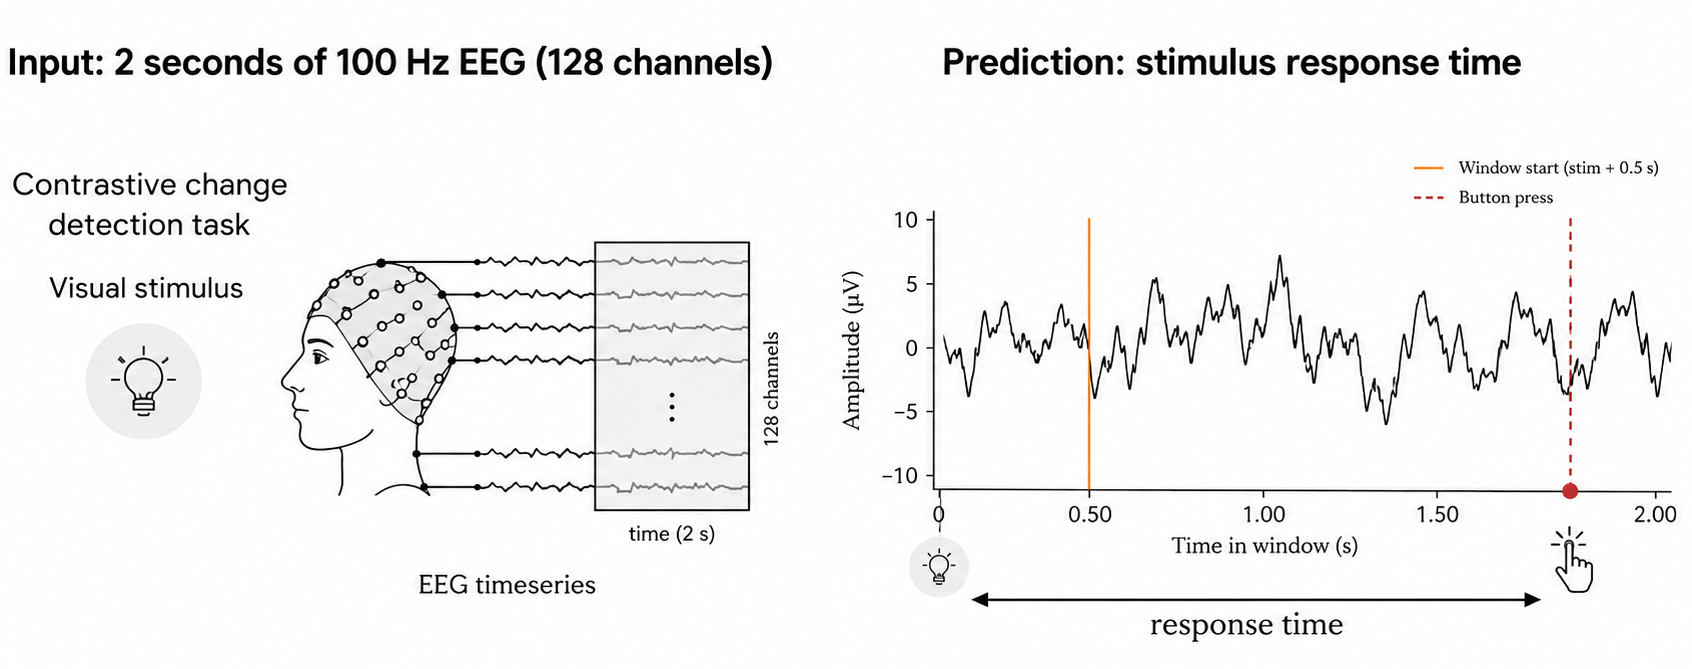
\includegraphics[width=0.9\linewidth]{img/challenge_task.png}
    \caption{HBN-EEG contrast change detection reaction-time task. Each trial provides a stimulus-locked EEG segment and a trial-wise RT target from stimulus onset to button press.}
    \label{fig:tasks}
\end{figure}


\subsection{Shared Evaluation Protocol}

We use this task as a controlled evaluation setting for separating three possible sources of RT prediction performance: EEG backbone capacity, temporal readout parameterization, and distributional event-time supervision. The benchmark therefore fixes the data split, target support, input representation, and scalar evaluation rule before varying architectures and objectives in the subsequent model and diagnostic sections.

To avoid subject leakage, all models use the same release-separated CCD split: R1--R8 for fitting, R9--R10 for development choices such as early stopping, checkpoint selection, readout-temperature tuning, and protocol diagnostics where applicable, and R11 for one-shot final reporting after all model and readout choices are fixed. R11 labels are not used for model fitting, checkpoint selection, readout-temperature selection, stacking, or protocol decisions. For consistency, the main analyzed set includes only trials whose response lies inside the fixed 2~s window (\(0.5 \leq \mathrm{RT} \leq 2.5\)~s). Table~\ref{tab:ccd_protocol_stats} reports the resulting partitions; metadata checks confirmed zero subject overlap across train, development, and R11 test after filtering.

\begin{table}[!t]
\centering
\caption{Release-separated CCD protocol statistics after window construction and RT-support filtering. Prepared trials are 2~s CCD windows with stimulus and response annotations; analyzed trials additionally satisfy \(0.5 \leq \mathrm{RT} \leq 2.5\)~s.}
\label{tab:ccd_protocol_stats}
\setlength{\tabcolsep}{3pt}
\renewcommand{\arraystretch}{1.12}
\begin{tabular*}{\linewidth}{@{\extracolsep{\fill}} l l r r r @{}}
\toprule
\textbf{Partition} & \textbf{Releases} & \textbf{Prepared trials} & \textbf{Analyzed trials} & \textbf{Subjects} \\
\midrule
Train & R1--R8 & 74{,}576 & 73{,}030 & 1{,}221 \\
Development & R9--R10 & 17{,}867 & 17{,}348 & 308 \\
Test & R11 & 15{,}751 & 15{,}164 & 292 \\
\bottomrule
\end{tabular*}
\end{table}

Scalar performance is evaluated using normalized RMSE (nRMSE), defined as RMSE divided by the standard deviation of the true targets within the evaluated split \citep{EEGChallengeWebsite2025}. Main scalar comparisons use the same support-filtered R9--R10 development set and R11 test set. Diagnostic analyses that require shifted crop starts, stricter RT support, posterior-only summaries, or stacking are introduced locally in the corresponding subsection or appendix and do not affect the main R11 model-selection protocol.

\subsection{Shared Training, Readout Tuning, and Inference Protocol}
\label{sec:shared_protocol}

To support this controlled comparison, we keep preprocessing, optimization, augmentation, checkpointing, and inference fixed wherever possible, so that the main experimental axes remain EEG backbone capacity, temporal readout parameterization, and distributional event-time supervision. All neural models receive the same input normalization: for each 2~s trial window and EEG channel, we subtract the channel's temporal mean within the window and divide by its temporal standard deviation within the same window. The shared training recipe uses Adam with learning rate \(10^{-3}\), zero weight decay, train batch size 128, up to 100 epochs, and early stopping on development nRMSE with patience 20.

Unless otherwise stated, training uses one fixed augmentation profile, so that regularization is not a model-specific tuning degree of freedom. The profile combines channel dropout, temporal cutout, and Gaussian noise with the same settings for all supervised neural models. Table~\ref{tab:shared_protocol_by_family} summarizes the remaining model-family-specific differences. Regression models use scalar RT supervision, while event-time models represent RT either as a soft crop-relative event-time target or as an observation under a latent event-time likelihood. When temperature scaling is used for event-time posterior readout, \(\tau\) is selected on R9--R10 to minimize development nRMSE of the posterior-mean readout and then applied unchanged to R11. The main regression-baseline and event-time-objective comparisons are repeated over five seeds (2025--2029).

\begin{table}[!t]
\centering
\caption{Model-family-specific targets and readouts within the shared protocol.}
\label{tab:shared_protocol_by_family}
\footnotesize
\setlength{\tabcolsep}{3pt}
\renewcommand{\arraystretch}{1.12}
\begin{tabularx}{\linewidth}{@{} >{\RaggedRight\arraybackslash}p{0.28\linewidth} >{\RaggedRight\arraybackslash}X >{\RaggedRight\arraybackslash}p{0.34\linewidth} @{}}
\toprule
\textbf{Model family} & \textbf{Target or supervision} & \textbf{Readout / tuning} \\
\midrule
Direct scalar regression & Scalar RT target. & Scalar RT output; segment-pooling MLP for MSP-CNN. \\
Temporal-readout regression & Scalar RT target or RT-derived readout loss. & Expected time over learned time-bin weights. \\
External EEG backbones & Scalar RT target; supervised from scratch. & Scalar RT output. \\
Soft-label event-time segmentation & Gaussian soft event-time target \(q(t)\). & Temperature-scaled posterior mean; \(\tau\) tuned on R9--R10. \\
EventNLL / likelihood variants & Observed RT under a latent event-time likelihood. & Temperature-scaled posterior mean; \(\tau\) tuned on R9--R10. \\
\bottomrule
\end{tabularx}
\end{table}

\section{Regression Controls}
\label{sec:regression_controls}

\subsection{Scalar Regression Baselines}

\label{sec:baseline_regression}

The regression baselines establish how far scalar supervision can go before introducing event-time targets. We separate two types of controls: compact task-specific temporal controls and supervised external EEG backbones trained from scratch under the same protocol.

The compact controls form a progression of window-level temporal inductive biases. MSP-CNN (multiscale segment-statistic pooling CNN; Figure~\ref{fig:ch1_regression}) explicitly accounts for temporal structure by collecting mean and max statistics from coarse temporal segments of the feature map. These segment-level summaries act as early/middle/late activation cues and are mapped to scalar RT. ETR-CNN (event-time readout CNN) turns this coarse temporal summary into a learned time-indexed readout: it preserves temporal scores over the input window and predicts RT as the expected time under learned time-bin weights. ETR-CNN large keeps the same readout while increasing feature capacity.

We compare these task-specific regressors with external EEG architectures adapted to scalar RT regression. These include classical convolutional EEG baselines, Deep4Net and ShallowFBCSPNet \citep{braindecode}; the compact EEGNet architecture \citep{lawhern2018eegnet}; TIDNet's thinker-invariant convolutional design \citep{kostas2020thinkerinvariance}; the convolutional-transformer EEGConformer \citep{song2023eegconformer}; the attention temporal convolutional ATCNet architecture \citep{altaheri2022atcnet}; EEGPT \citep{wang2024eegpt}; Medformer \citep{wang2024medformer}; and the LaBraM foundation-style architecture \citep{Jiang2024LaBraM}. All external architectures are trained from scratch; pretrained weights are not used.

ETR-CNN large is the strongest scalar baseline, with MSP-CNN and base ETR-CNN close behind. The external EEG backbones train meaningfully but do not close the gap to these compact temporal controls, suggesting that task-specific temporal structure matters more for this RT task than generic backbone capacity alone. These results provide strong scalar controls for the next step: testing whether directly supervising an event-time distribution improves beyond scalar RT training.

\begin{table}[!t]
\centering
\caption{Direct-regression and wrapped external backbone baselines. Values are mean $\pm$ sample standard deviation.}
\label{tab:r11_regression_baselines}
\footnotesize
\setlength{\tabcolsep}{2pt}
\renewcommand{\arraystretch}{1.15}
\begin{tabularx}{\linewidth}{@{} >{\RaggedRight\arraybackslash}p{0.22\linewidth} Y >{\centering\arraybackslash}p{0.215\linewidth} >{\centering\arraybackslash}p{0.215\linewidth} @{}}
\toprule
\textbf{Model} & \textbf{Role} & \textbf{Valid nRMSE} $\downarrow$ & \textbf{R11 nRMSE} $\downarrow$ \\
\midrule
\multicolumn{4}{@{}l}{\textit{Task-specific regression baselines}} \\
\addlinespace[0.15em]
MSP-CNN & segment-pooling scalar & \mbox{0.9006 $\pm$ 0.0051} & \mbox{0.8998 $\pm$ 0.0080} \\
ETR-CNN & temporal readout & \mbox{0.9008 $\pm$ 0.0060} & \mbox{0.8977 $\pm$ 0.0068} \\
ETR-CNN large & capacity ablation & \mbox{0.8972 $\pm$ 0.0040} & \mbox{0.8928 $\pm$ 0.0042} \\
\midrule
\multicolumn{4}{@{}l}{\textit{External regression baselines}} \\
\addlinespace[0.15em]
TIDNet & thinker-invariant CNN & \mbox{0.9235 $\pm$ 0.0024} & \mbox{0.9192 $\pm$ 0.0027} \\
EEGConformer & conv-transformer & \mbox{0.9188 $\pm$ 0.0026} & \mbox{0.9287 $\pm$ 0.0057} \\
EEGNet & compact CNN & \mbox{0.9350 $\pm$ 0.0054} & \mbox{0.9335 $\pm$ 0.0028} \\
LaBraM & foundation-style & \mbox{0.9304 $\pm$ 0.0061} & \mbox{0.9327 $\pm$ 0.0086} \\
Deep4Net & deep ConvNet & \mbox{0.9269 $\pm$ 0.0045} & \mbox{0.9260 $\pm$ 0.0044} \\
ShallowFBCSPNet & shallow FBCSP CNN & \mbox{0.9324 $\pm$ 0.0016} & \mbox{0.9343 $\pm$ 0.0024} \\
ATCNet & conv/attention/TCN & \mbox{0.9686 $\pm$ 0.0183} & \mbox{0.9666 $\pm$ 0.0151} \\
EEGPT & foundation-style & \mbox{0.9616 $\pm$ 0.0201} & \mbox{0.9584 $\pm$ 0.0185} \\
Medformer & larger transformer & \mbox{0.9623 $\pm$ 0.0046} & \mbox{0.9585 $\pm$ 0.0051} \\
\bottomrule
\end{tabularx}
\end{table}

\begin{figure}[!t]
    \centering
    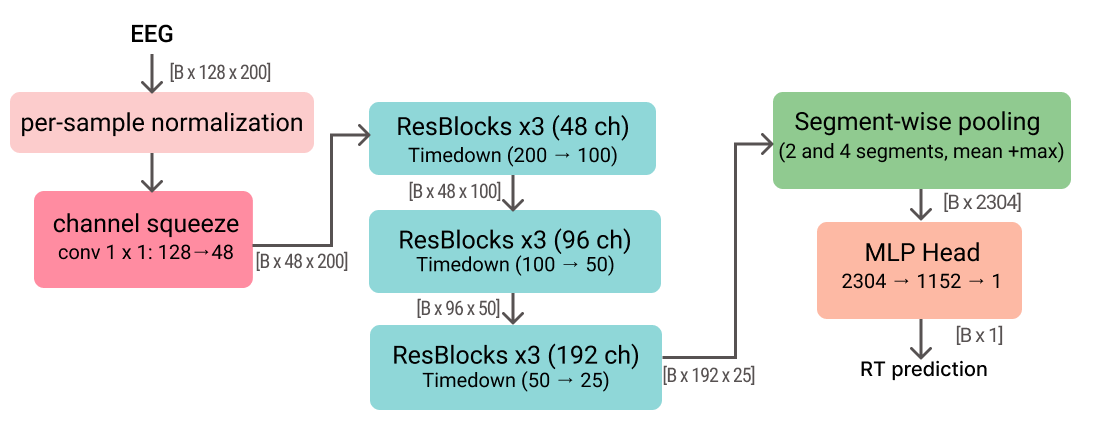
\includegraphics[width=\linewidth]{img/ch1/Ch1_regression.png}
    \caption{MSP-CNN direct RT regression baseline architecture. A lightweight 1-D temporal ConvNet maps an EEG trial window to a scalar reaction-time prediction. A learned $1\times1$ channel-squeeze layer (128$\rightarrow$48) is followed by residual depthwise-separable stages with anti-aliased temporal downsampling, segment-wise pooling (2 and 4 segments; mean+max), and an MLP head.}
    \label{fig:ch1_regression}
\end{figure}

\section{Event-Time Posterior Formulation}
\label{sec:event_time_formulation}

To make response timing explicit, we reformulate RT prediction as event-time posterior modeling. Instead of predicting a scalar directly, the model produces per-time logits and a posterior distribution over response-relevant event times; scalar RT is then read out as the posterior expectation. The key distinction from temporal-readout regression is that the objective directly supervises the distributional event-time representation, rather than using a temporal head only as a scalar-regression readout.

We evaluate two ways of turning scalar RT labels into event-time supervision. The first constructs an explicit soft target distribution over time, asking the model to match a smoothed target centered at the observed RT. The second treats the observed RT statistically, as a noisy observation of an unobserved response-relevant event time, and optimizes a latent event-time likelihood. These two families correspond to soft-target objectives and likelihood-based objectives, respectively.

The core event-time experiments are designed to isolate the role of output formulation. The regression controls above test how far scalar supervision can go with task-specific temporal readouts and external EEG backbones. Here, we fix the event-time segmentation U-Net (ETS-U-Net) backbone and vary the event-time objective, so that differences in scalar accuracy, posterior geometry, and diagnostic behavior under temporal crop shifts reflect how RT is supervised over time rather than which architecture is used.

\subsection{Event-Time Segmentation Architecture}
\label{sec:event_time_architectures}

ETS-U-Net maps an EEG trial window
$X\in\mathbb{R}^{C\times T}$ to per-time logits $z_{0:T-1}$ (Figure~\ref{fig:ets_unet}). It follows a 1-D U-Net style encoder-decoder with skip
connections for precise localization \citep{ronneberger2015unet}. The encoder progressively downsamples the temporal axis
to build multi-scale context, while the decoder upsamples and fuses encoder features to recover per-time outputs at the
input temporal resolution (internal down/up-sampling is used only to form multi-scale features). Each scale is refined
with lightweight residual blocks (ResNet-style skips) \citep{he2016resnet} built from depthwise-separable 1-D convolutions
for computational efficiency \citep{howard2017mobilenets,chollet2017xception}. To mitigate aliasing under temporal
decimation, downsampling applies a fixed depthwise smoothing filter followed by strided averaging (``blur-pool'' style)
\citep{zhang2019shiftinvariant}. A dilated bottleneck further enlarges the receptive field without additional downsampling
\citep{yu2016dilated}.

\begin{figure}[t]
    \centering
    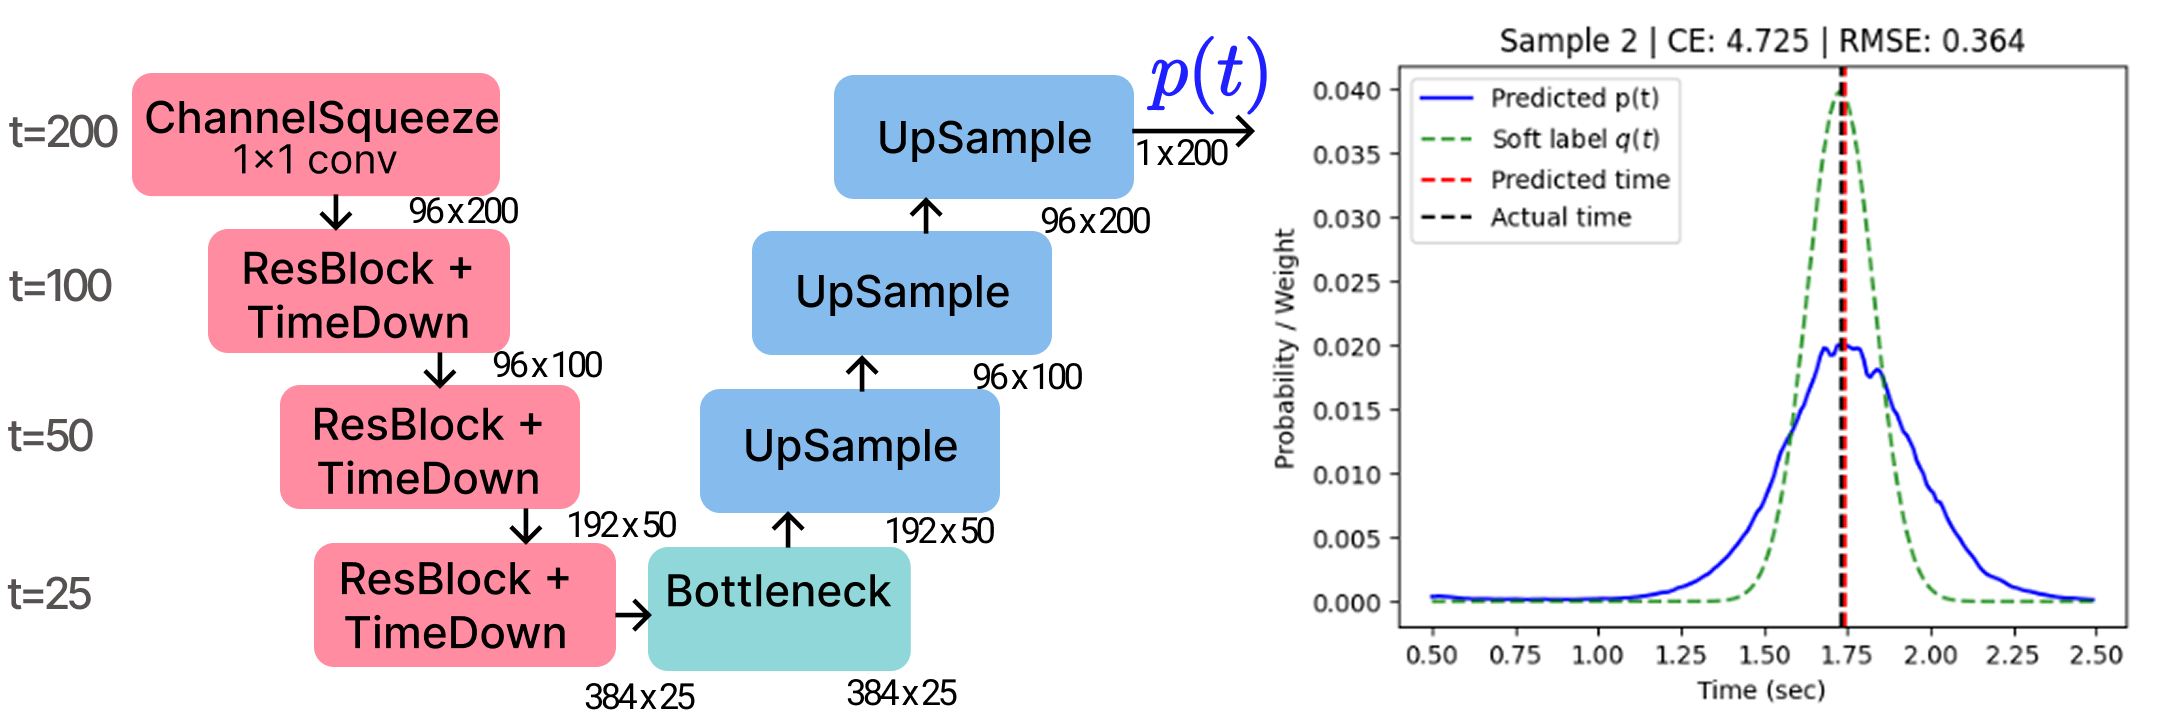
\includegraphics[width=0.9\linewidth]{img/ch1/Ch1_ets_unet_1.png}
    \caption{ETS-U-Net for RT segmentation. A lightweight 1-D U-Net maps an EEG trial window to per-time logits
    and an event-time distribution $p(t)$. The encoder applies a $1\times1$ channel-squeeze layer followed by residual
    blocks with temporal downsampling (\texttt{TimeDown}); a bottleneck aggregates context, and the decoder upsamples with
    skip connections to recover time-resolved outputs. The right panel shows an example prediction $p(t)$ and Gaussian soft
    target $q(t)$, together with the resulting predicted vs.\ observed response time.}
    \label{fig:ets_unet}
\end{figure}

\subsection{Soft-Target Event-Time Objectives}

Soft-target objectives instantiate the direct-supervision route: the observed RT is converted into a smooth target distribution over the represented time grid.

\paragraph{Soft target distribution.}
For each fixed 2~s input window, the observed RT \(y\) is converted into a
window-relative temporal target \(y_{\mathrm{rel}}=y-0.5\)~s on the represented
time grid.
A smooth segmentation label is constructed using a Gaussian kernel with bandwidth $\sigma$:
\begin{equation}
\label{eq:rt_soft_target}
\tilde q_t=\exp\left(-\frac{(g_t-y_{\mathrm{rel}})^2}{2\sigma^2}\right),\qquad
q_t=\frac{\tilde q_t}{\sum_{k=0}^{T-1}\tilde q_k},\qquad
\sum_{t=0}^{T-1} q_t=1.
\end{equation}
The Gaussian label avoids a degenerate single-bin target while keeping probability mass concentrated near the observed behavioral latency.

\paragraph{Model output and losses.}
Given logits $z_t$ for $t=0,\dots,T-1$, the predicted event-time distribution is obtained via temperature-scaled softmax,
\begin{equation}
\label{eq:rt_pred_dist}
p_t(\tau)=\frac{e^{z_t/\tau}}{\sum_{k=0}^{T-1} e^{z_k/\tau}}.
\end{equation}
The soft-label segmentation family is written as a weighted objective:
\begin{equation}
\label{eq:rt_loss}
\begin{aligned}
\mathcal{L}
&= \lambda_{\text{time}}\,\mathrm{RMSE}\big(\hat t_{\mathrm{rel}}(\tau), y_{\mathrm{rel}}\big)
 + \lambda_{\text{CE}}\,\mathrm{CE}\big(q, p(\tau)\big) \\
&\quad + \lambda_{W1}\,W_1\big(\mathrm{CDF}(q), \mathrm{CDF}(p(\tau))\big)
 + \lambda_{\text{KL}}\,D_{\mathrm{KL}}\big(q\|p(\tau)\big)
 + \lambda_{H}\,H\big(p(\tau)\big),
\end{aligned}
\end{equation}
where  
\begin{equation*}
\mathrm{CE}(q,p)=-\sum_{t=0}^{T-1} q_t \log p_t, \;
D_{\mathrm{KL}}(q\|p)=\sum_{t=0}^{T-1} q_t \log\frac{q_t}{p_t}, \;
H(p)=-\sum_{t=0}^{T-1} p_t \log p_t.
\end{equation*}
This expression defines an ablation family rather than a single prescribed loss. CE-only supervision sets the scalar time term to zero and asks the model to match a Gaussian soft event-time label. The time-only ablation removes distributional matching while keeping the same readout, and the Wasserstein-only ablation tests whether a CDF-based geometry loss is sufficient on its own. A CE+time hybrid is available by enabling both CE and soft-argmax time terms, but is not a separate row in the five-seed comparison. Entropy, KL, focal, and related terms serve as posterior-geometry controls when enabled.

\subsection{Likelihood-Based Event-Time Objectives}
\label{sec:event_nll}

As a probabilistic alternative to soft-target supervision, likelihood-based objectives model the observed scalar RT as a noisy realization of a latent event time. Given the posterior over latent event bins, the marginal likelihood of the observed RT is
\begin{equation}
\label{eq:event_nll}
p(y\mid X)
= \sum_{t=0}^{T-1} p_t(X)\,
\mathcal{N}\!\left(y;\,t_0 + g_t,\,\sigma_y^2\right),
\qquad
\mathcal{L}_{\mathrm{EventNLL}} = -\log p(y\mid X).
\end{equation}
This objective keeps the same event-time interpretation but replaces the constructed target distribution $q_t$ with a marginal likelihood over latent response-relevant event times.

\paragraph{Observation-kernel and hazard extensions.}
The EventNLL formulation separates the latent event-time posterior $p_t(X)$ from the observation model $K(y\mid t)$. The default model uses a single Gaussian observation kernel, but we also evaluate a two-scale Gaussian mixture,
\begin{equation}
\label{eq:event_nll_mixture_kernel}
K(y\mid t)=(1-\alpha)\,\mathcal{N}(y;t_0+g_t,\sigma_{\mathrm{narrow}}^2)
+\alpha\,\mathcal{N}(y;t_0+g_t,\sigma_{\mathrm{wide}}^2),
\end{equation}
which keeps most probability mass in a narrow timing error while allowing a wider tail for occasional noisy RT observations. In the completed run, $\sigma_{\mathrm{narrow}}=0.10$~s, $\sigma_{\mathrm{wide}}=0.35$~s, and $\alpha=0.10$.

As a readout extension, we also evaluate a hazard/survival parameterization. Instead of using logits only as unconstrained softmax scores, each temporal logit defines a conditional event probability
\begin{equation}
\label{eq:hazard_readout}
h_t=\sigma(z_t/\tau),\qquad
p_t^{\mathrm{haz}} \propto h_t\prod_{k<t}(1-h_k),
\end{equation}
with the resulting event-bin probabilities normalized over the represented window. This keeps the same event-time likelihood in Eq.~\ref{eq:event_nll}, but changes the posterior parameterization from a categorical softmax to a discrete-time survival process. This extension tests whether the event-time formulation is tied to one softmax implementation.

\subsection{Formulation Comparison and Robustness}
Table~\ref{tab:r11_segmentation_losses} compares the paper-facing ETS-U-Net objective variants under the fixed backbone and release-separated protocol. Here, R11 \(\tau\)-nRMSE denotes R11 nRMSE after applying the posterior-readout temperature \(\tau\) selected on R9--R10; R11 labels are used only for evaluation. The CE and likelihood-family objectives form the strongest scalar-readout group after readout-temperature tuning, with R11 \(\tau\)-nRMSE between 0.8745 and 0.8778. This improves over the strongest scalar regression baseline, ETR-CNN large (0.8928 $\pm$ 0.0042; Table~\ref{tab:r11_regression_baselines}), while the time-only and Wasserstein controls remain closer to the scalar-regression regime.

\begin{table}[!t]
\centering
\caption{Event-time objective variants with a fixed ETS-U-Net backbone. Values are mean $\pm$ sample standard deviation.}
\label{tab:r11_segmentation_losses}
\footnotesize
\setlength{\tabcolsep}{2pt}
\renewcommand{\arraystretch}{1.15}
\begin{tabularx}{\linewidth}{@{} >{\RaggedRight\arraybackslash}p{0.22\linewidth} Y >{\centering\arraybackslash}p{0.18\linewidth} >{\centering\arraybackslash}p{0.18\linewidth} >{\centering\arraybackslash}p{0.18\linewidth} @{}}
\toprule
\textbf{Model} & \textbf{Variant} & \textbf{Valid nRMSE} $\downarrow$ & \textbf{R11 nRMSE} $\downarrow$ & \textbf{R11 \(\tau\)-nRMSE} $\downarrow$ \\
\midrule
\multicolumn{5}{@{}l}{\textit{Soft-target objective}} \\
\addlinespace[0.15em]
CE & soft target & \mbox{0.8763 $\pm$ 0.0044} & \mbox{0.8774 $\pm$ 0.0044} & \mbox{0.8753 $\pm$ 0.0039} \\
\midrule
\multicolumn{5}{@{}l}{\textit{Likelihood-based objectives}} \\
\addlinespace[0.15em]
EventNLL & Gaussian kernel & \mbox{0.8769 $\pm$ 0.0030} & \mbox{0.8805 $\pm$ 0.0021} & \mbox{0.8772 $\pm$ 0.0018} \\
Mixture EventNLL & two-scale kernel & \mbox{0.8744 $\pm$ 0.0018} & \mbox{0.8785 $\pm$ 0.0047} & \mbox{0.8745 $\pm$ 0.0053} \\
Hazard EventNLL & hazard readout & \mbox{0.8755 $\pm$ 0.0027} & \mbox{0.8776 $\pm$ 0.0031} & \mbox{0.8778 $\pm$ 0.0041} \\
\midrule
\multicolumn{5}{@{}l}{\textit{Readout and distance controls}} \\
\addlinespace[0.15em]
Time-only & scalar time loss & \mbox{0.8944 $\pm$ 0.0048} & \mbox{0.8943 $\pm$ 0.0025} & \mbox{0.8917 $\pm$ 0.0046} \\
Wasserstein & CDF loss & \mbox{0.8997 $\pm$ 0.0035} & \mbox{0.8995 $\pm$ 0.0078} & \mbox{0.8896 $\pm$ 0.0033} \\
\bottomrule
\end{tabularx}
\end{table}

\paragraph{Objective ablations.}
The ablations separate expectation-style temporal readout from distributional supervision. The time-only model directly optimizes soft-argmax error but removes distribution matching; it remains close to the strongest scalar-regression baseline and trails the CE/EventNLL group by roughly 0.014--0.017 R11 \(\tau\)-nRMSE. CE and the likelihood-family variants form a tight top group: mixture EventNLL has the best mean temperature-tuned scalar readout, but CE, Gaussian EventNLL, mixture EventNLL, and hazard EventNLL are close relative to seed variability. The hazard result shows that the likelihood-family conclusion is not tied to a categorical softmax posterior, while the Wasserstein control shows that an alternative distributional distance alone does not match the strongest scalar readouts. Thus, the central gain is best attributed to distributional event-time supervision rather than to the U-Net backbone or soft-argmax readout alone.

\section{Posterior Readout and Diagnostics}
\label{sec:posterior_diagnostics}

\subsection{Posterior Geometry and Readout Temperature Tuning}

The posterior view makes geometric properties of the predicted distribution directly inspectable. CDF-based distances penalize temporal displacement of probability mass, entropy and variance summarize posterior sharpness, and quantiles expose asymmetric uncertainty around the predicted response time. These summaries are useful for diagnosis and for downstream stacking.

When used, explicit posterior regularization can be written generically as
\begin{equation}
\label{eq:posterior_regularized_objective}
\mathcal{L} = \mathcal{L}_{\mathrm{event}} + \lambda R\!\left(p(t\mid X)\right),
\end{equation}
where $R$ may target entropy, variance, tail mass, or other posterior-shape statistics. Here, such terms are used as posterior-geometry controls unless they are explicitly evaluated as ablations.

\paragraph{Inference and temperature tuning.}
The relative event time is estimated by expectation (soft-argmax),
\begin{equation}
\label{eq:rt_soft_argmax}
\hat t_{\mathrm{rel}}(\tau)=\sum_{t=0}^{T-1} p_t(\tau)\, g_t,
\qquad
\hat t_{\mathrm{abs}}(\tau)=t_0+\hat t_{\mathrm{rel}}(\tau),
\end{equation}
where $g_t=t\,\Delta t$ denotes the discrete time grid. Under squared error, the Bayes-optimal point estimate is the
conditional mean; accordingly, reading out RT by $\mathbb{E}_{p(t)}[g]$ aligns naturally with the nRMSE objective (RMSE
up to a constant normalization).

In practice, different training choices (loss weighting, augmentation strength, and checkpoint selection) produced
time-distributions with markedly different sharpness and entropy: some models generated very peaked $p(t)$ while others
were systematically more diffuse. This creates a confidence-scale mismatch, where naive averaging (or stacking without
temperature-scaled inputs) can underweight accurate but underconfident models and overweight overconfident ones.

We therefore use post-hoc temperature scaling \citep{guo2017calibration} to tune the softness of $p(t)$, improving the
readout and making confidence profiles more comparable across losses and models.
Temperature is selected by validation tuning for each base model $m$:

\begin{equation}
\label{eq:rt_tau_tuning}
\tau_m^\star = \arg\min_{\tau\in\mathcal{T}_{\text{cal}}}
\ \mathrm{nRMSE}_{\text{val}}\big(\hat t_{\mathrm{abs}}^{(m)}(\tau)\big).
\end{equation}

Under the release-separated protocol, $\mathcal{T}_{\text{cal}}$ is selected on the R9-R10 development split and applied unchanged to R11.

Because confidence scales differ across objectives and architectures, temperature is treated as a posterior-geometry
control selected on development data rather than as a separate model-selection signal.

\paragraph{Posterior geometry and interval coverage.}
The scalar comparisons above compare models through the posterior mean, but the event-time formulation produces a full distribution over response latencies. Two losses can therefore have similar nRMSE while assigning probability mass very differently over time. We analyze this posterior geometry to ask whether the scalar prediction is supported by a localized temporal event distribution, whether the posterior is overly diffuse or overly concentrated, and whether nominal posterior intervals have meaningful empirical coverage.

For this analysis, the softmax temperature is selected on R9--R10 to minimize scalar nRMSE of the posterior-mean readout. Thus, we treat temperature selection as readout-temperature tuning rather than as full probabilistic calibration. After this readout tuning, we evaluate the learned event-time posterior itself: whether its mass is near the observed RT, whether the posterior mean agrees with the posterior mode, and whether nominal posterior intervals contain the true RT at the expected rate.

Figure~\ref{fig:posterior_raster_main} provides a trial-sorted view of these posteriors before reducing them to summary metrics. It shows how each loss distributes probability mass across the represented RT range, making posterior width, target alignment, and loss-specific confidence patterns visible at the dataset level.

Table~\ref{tab:posterior_geometry_metrics} uses four groups of metrics. First, scalar nRMSE and MAE measure the posterior-mean RT prediction. Second, CRPS and fixed-kernel EventNLL score the full posterior distribution; lower values indicate better distributional predictions. The fixed-kernel EventNLL uses the same Gaussian observation kernel for all models, so it evaluates the predicted event-time distribution under a common likelihood score rather than under each model's own training loss. Third, Width80, Mass $\pm$150 ms, and mode-mean gap describe posterior geometry: Width80 is the median width of the nominal 80\% central posterior interval, Mass $\pm$150 ms is the posterior probability assigned within 150 ms of the observed RT, and mode-mean gap measures disagreement between the posterior peak and the posterior mean used for scalar readout. Finally, Coverage80 and Coverage MAE summarize interval coverage. Coverage80 is the empirical coverage of the nominal 80\% central interval, whose calibrated target is 0.80. Coverage MAE is the mean absolute difference between empirical and nominal coverage over central intervals $\{50\%,60\%,70\%,80\%,90\%\}$.

\begin{figure}[!t]
    \centering
    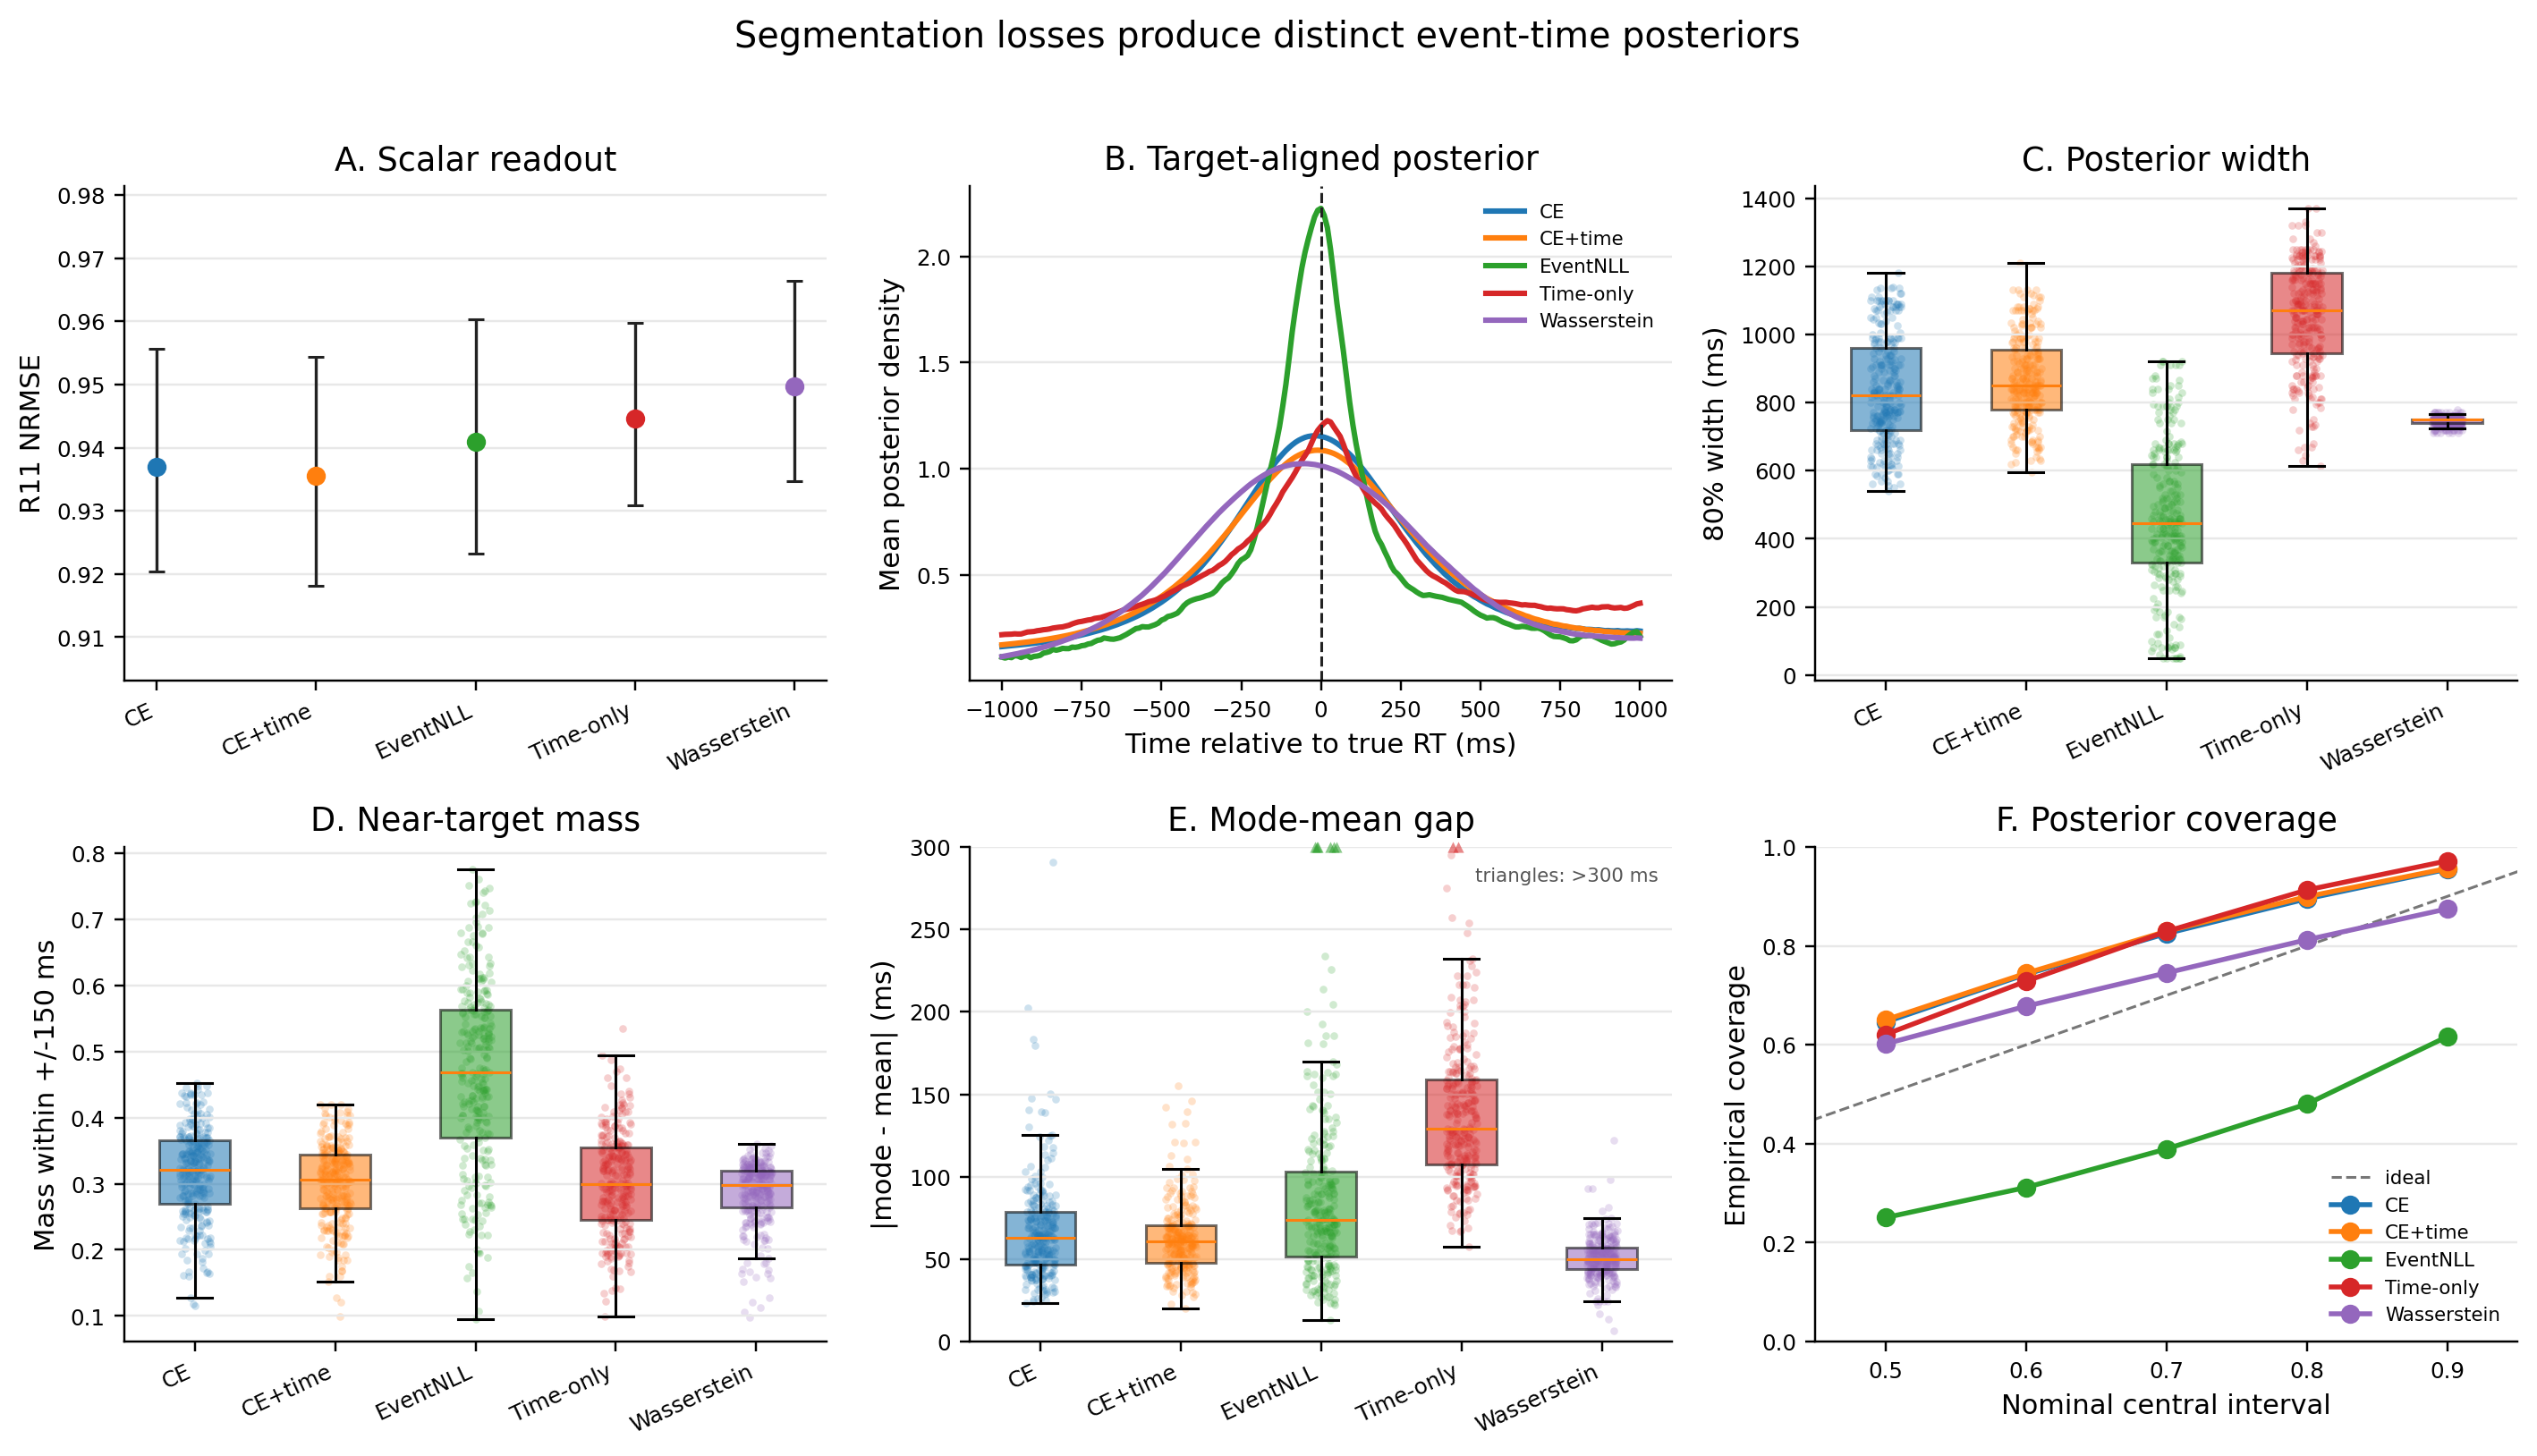
\includegraphics[width=\linewidth]{img/ch1/posterior_geometry_main_calibrated.png}
    \caption{Posterior geometry differs across event-time losses even when scalar nRMSE is similar. Panel A reports R11 scalar readout after selecting the softmax temperature on R9--R10 to minimize nRMSE. Panel B aligns predicted posteriors to the true RT. Panels C--E summarize posterior width, near-target mass, and mode-mean disagreement. Panel F compares empirical coverage of central posterior intervals; the diagonal is ideal interval coverage.}
    \label{fig:posterior_geometry_main}
\end{figure}

\begin{figure}[!t]
    \centering
    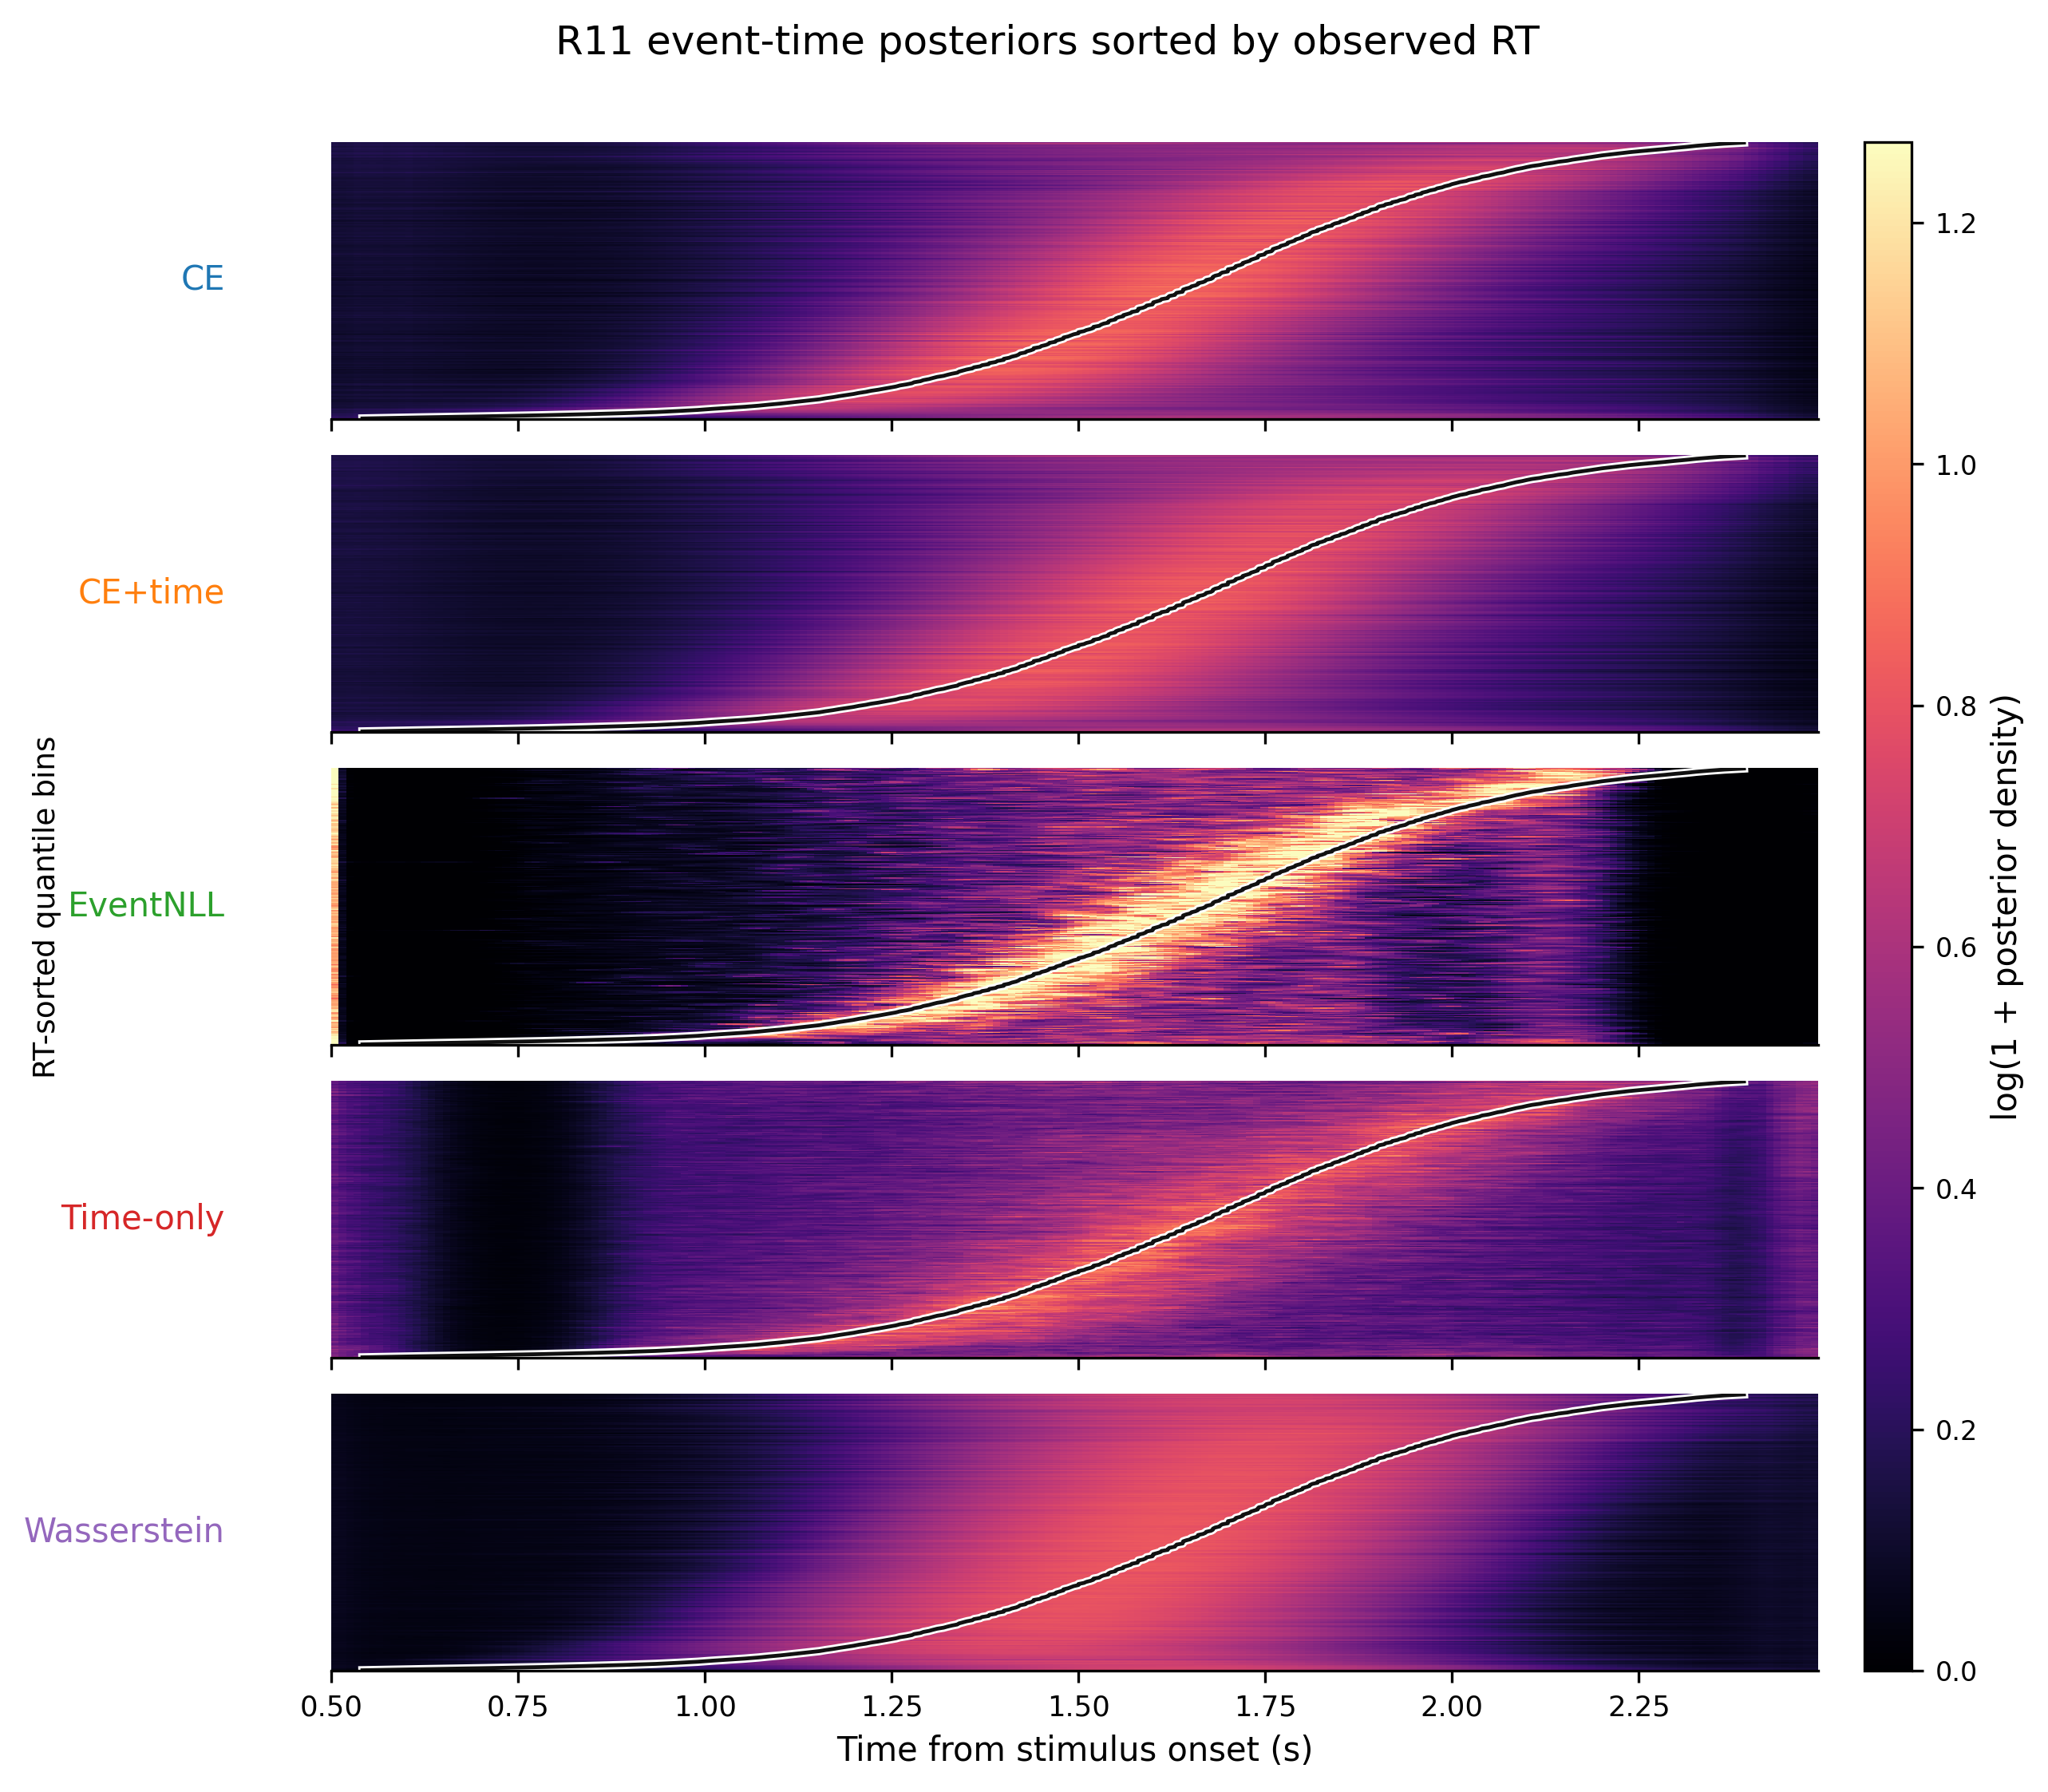
\includegraphics[width=\linewidth]{img/ch1/trial_sorted_posterior_raster_calibrated.png}
    \caption{Trial-sorted event-time posterior maps on R11 for matched segmentation losses. Rows are quantile bins of representable R11 trials sorted by observed RT; the x-axis is time from stimulus onset; color shows log-transformed posterior density averaged within each bin. The black curve marks the mean observed RT in each bin.}
    \label{fig:posterior_raster_main}
\end{figure}

\begin{table}[!t]
\centering
\caption{Quantitative posterior geometry on R11 for matched event-time segmentation losses. Metrics are defined in the text. CRPS is reported in milliseconds. Fixed-kernel EventNLL uses a common Gaussian observation kernel for all models ($\sigma=0.15$~s). For Coverage80, values closer to 0.80 indicate better nominal 80\% interval coverage; for Coverage MAE, lower is better.}
\label{tab:posterior_geometry_metrics}
\scriptsize
\setlength{\tabcolsep}{3pt}
\renewcommand{\arraystretch}{1.12}
\resizebox{\linewidth}{!}{%
\begin{tabular}{@{} l c c c c c c c c c @{}}
\toprule
\textbf{Model} & \textbf{nRMSE} & \textbf{MAE ms} & \textbf{CRPS ms} & \textbf{Fixed NLL} & \textbf{Width80 ms} & \textbf{Mass $\pm$150 ms} & \textbf{Mode-mean gap ms} & \textbf{Coverage80} & \textbf{Coverage MAE} \\
\midrule
CE & 0.937 & 216 & 155 & 0.115 & 820 & 0.328 & 57 & 0.895 & 0.113 \\
CE+time & 0.936 & 219 & 157 & 0.144 & 860 & 0.311 & 57 & 0.899 & 0.116 \\
EventNLL & 0.941 & 216 & 162 & -0.027 & 450 & 0.487 & 72 & 0.480 & 0.290 \\
Time-only & 0.945 & 228 & 167 & 0.203 & 1070 & 0.311 & 129 & 0.913 & 0.113 \\
Wasserstein & 0.950 & 222 & 165 & 0.219 & 740 & 0.296 & 50 & 0.812 & 0.053 \\
\bottomrule
\end{tabular}%
}
\end{table}

These metrics show that the losses induce different output semantics. CE+time and CE give the strongest scalar readouts, but their nominal 80\% intervals cover about 90\% of trials, indicating conservative over-coverage. EventNLL is not well calibrated as an uncertainty posterior: its nominal 80\% interval covers only 48\% of trials. Its value is instead localization-like concentration, with the narrowest Width80, the highest near-target mass, and the best fixed-kernel EventNLL score. Wasserstein has the smallest Coverage MAE and a Coverage80 value closest to 0.80, but this comes with weaker scalar nRMSE and lower near-target mass. Thus, posterior geometry reveals a trade-off among scalar accuracy, target concentration, and interval coverage that is hidden by nRMSE alone.

\paragraph{Secondary ensemble use of posterior features.}
The same posterior summaries can also serve as post-hoc ensemble features, but we treat this as a secondary analysis rather than as a main release-separated claim. The single-model R11 comparisons above are intentionally reported without stacking, so that the main evidence isolates the event-time objective, scalar readout, posterior geometry, and the shifted-crop diagnostic below. The stacker construction is described in Appendix~\ref{sec:rt_stacking}; in the original hidden-release CodaBench evaluation (Appendix Table~\ref{tab:appendix_codabench}), gradient boosting stacking achieved 0.91394 hidden nRMSE, compared with 0.92334 for the best single model, 0.91840 for manual blending, and 0.91539 for Ridge stacking. This supports posterior-derived meta-features as an ensemble calibration layer while keeping the paper's main claims tied to single-model release-separated analyses.

\subsection{Shifted-Crop Localization Diagnostic}

The posterior analyses above show that event-time losses produce different probability geometries, but they do not by themselves prove that a model has learned a within-crop event localizer. A fixed stimulus-locked window can still permit shortcut behavior: a model may predict trial difficulty, subject-level slowness, or stimulus-locked response tendency without moving its prediction when the crop is shifted. We therefore introduced a shifted-crop diagnostic on R11 using the trained models and R9--R10-selected temperatures. For each trial, we used the same 5~s EEG cache and evaluated the model on 2~s crops starting at $s\in\{0.2,0.3,\dots,0.8\}$~s. The reference crop is $s=0.5$~s, matching the training and main inference protocol. To avoid target-censoring effects, this analysis uses the common-inside subset where RT remains inside all shifted crops ($0.8\leq \mathrm{RT}\leq 2.2$~s; 14{,}183 trials).

If the model truly localizes the response-relevant event within the crop, shifting the crop start by $\Delta s$ should move the predicted crop-relative event time by approximately $-\Delta s$, giving a raw shift slope near $-1$. A crop-invariant scalar regressor should instead have a slope near 0. Table~\ref{tab:shifted_crop_diagnostic} shows that the event-time segmentation models preserve or improve reference-crop accuracy and move in a more localizer-like direction than the best scalar regressor. EventNLL reaches a raw shift slope of $-0.292$ [95\% CI: $-0.311$, $-0.272$], compared with $-0.253$ [$-0.270$, $-0.235$] for ETR-CNN and $-0.172$ on average across regression baselines. The fraction of localizer-like trials also increases from 10.1\% for ETR-CNN to 14.8\% for CE and 15.9\% for EventNLL.

This result should be interpreted as evidence for a representational shift, not as solved shift equivariance. The segmentation models remain far from the ideal slope of $-1$, indicating that fixed-window training still mixes event localization with scalar response-tendency shortcuts. That limitation is useful: it identifies shift-augmented, crop-relative event-time training as the natural next step if the goal is a stronger trial-wise neural event localizer.

\begin{table}[!t]
\centering
\caption{Shifted-crop diagnostic on the R11 common-inside subset. The ideal within-crop event localizer has raw shift slope $-1$; a crop-invariant scalar shortcut has slope 0. Reference nRMSE is computed at the standard $s=0.5$~s crop.}
\label{tab:shifted_crop_diagnostic}
\scriptsize
\setlength{\tabcolsep}{3pt}
\renewcommand{\arraystretch}{1.12}
\resizebox{\linewidth}{!}{%
\begin{tabular}{@{} l c c c c c c @{}}
\toprule
\textbf{Model} & \textbf{Ref nRMSE} $\downarrow$ & \textbf{Ref MAE, s} $\downarrow$ & \textbf{Worst $\Delta$ nRMSE} & \textbf{Raw shift slope} & \textbf{Localizer-like trials} & \textbf{Invariant-like trials} \\
\midrule
ETR-CNN & 0.874 & 0.206 [0.199, 0.215] & 0.174 & $-0.253$ [$-0.270$, $-0.235$] & 10.1\% [9.0, 11.1] & 34.5\% \\
ETS-U-Net CE & 0.856 & 0.201 [0.193, 0.209] & 0.193 & $-0.287$ [$-0.306$, $-0.267$] & 14.8\% [13.3, 16.3] & 34.4\% \\
ETS-U-Net EventNLL & 0.859 & 0.201 [0.193, 0.210] & 0.198 & $-0.292$ [$-0.311$, $-0.272$] & 15.9\% [14.5, 17.3] & 33.3\% \\
\bottomrule
\end{tabular}%
}
\end{table}

\section{Discussion}

\subsection{RT Prediction as Event-Time Localization}

The results support treating trial-wise RT prediction as event-time localization rather than as ordinary scalar regression. The label is the latency of a response within a post-stimulus interval, and models benefit when that timing structure is explicit in both the output space and the loss. The shifted-crop diagnostic adds a stricter check on this interpretation: event-time segmentation models move in a more event-like direction than scalar regression under temporal crop shifts, but their slopes remain far from perfect localizer behavior. This framing therefore connects naturally to response-locked EEG analyses while also making clear that fixed-window RT prediction is not the same as fully shift-equivariant event detection.

\subsection{Why Distributional Supervision Helps}

Distributional supervision gives the model a local temporal target instead of a single global scalar penalty. CE-only and hybrid losses outperform the time-only loss, suggesting that the gain is not just a differentiable soft-argmax readout. The soft event-time target encourages probability mass near plausible response latencies and makes label-consistent shifted-crop diagnostics or future crop-jitter variants well defined. EventNLL reaches a similar scalar-error regime through a different route: it marginalizes a latent event time instead of asking the model to imitate a hand-constructed Gaussian mask.

\subsection{Relation to EEG Backbones and Pretraining}

The wrapped external baselines show that standard EEG architectures can train under the fixed normalization protocol, but they do not close the gap to compact task-specific models or event-time segmentation. Foundation-style architectures are evaluated here as architectures trained from scratch, not as pretrained models. The comparison is therefore not a test of pretraining; it shows that, under this benchmark protocol, formulation and objective design are strong levers even with lightweight supervised models.

\subsection{Why Posterior Geometry Matters}

The event-time posterior contains more information than its expectation. Sharpness, entropy, variance, quantiles, and the gap between posterior mode and posterior mean describe confidence and ambiguity in ways that scalar predictions discard. The posterior analysis shows that CE, CE+time, EventNLL, time-only, and Wasserstein losses can have similar scalar readouts but different target-alignment, width, and coverage behavior. Temperature calibration is therefore best understood as posterior-geometry control and a fairness step for comparing readouts, not as the main methodological claim.

\subsection{Limitations}

The main limitation is that all claims are tied to HBN-EEG CCD and the release-separated protocol used here. R11 is a stronger local holdout than reused validation performance, but it is still drawn from the same broader dataset family and preprocessing pipeline. The shifted-crop diagnostic shows partial localization, not full shift equivariance, so stronger claims about trial-wise neural event localization would require training protocols that explicitly randomize crop position and supervise crop-relative timing. The five-seed robustness checks support the main scalar-versus-event-time comparison, but they cover selected core recipes rather than every kernel, hazard, calibration, and architecture variant. The foundation-style comparisons also do not use pretrained weights or montage-specialized setup changes; they are controlled architecture baselines rather than a full evaluation of EEG foundation models.

\section{Conclusion}

We reformulated EEG-based reaction-time prediction as event-time distribution modeling and evaluated it under a release-separated HBN-EEG protocol. The results indicate that supervising an event-time posterior improves RT prediction beyond scalar regression and beyond a temporal-readout head alone. Loss ablations and five-seed robustness checks show that distributional event-time supervision matters, EventNLL provides a principled latent-variable likelihood alternative, and posterior-geometry plus shifted-crop analyses reveal output behavior that scalar nRMSE alone cannot capture.

\appendix

\section{Distribution-Aware Stacking}
\label{sec:rt_stacking}
Segmentation-style outputs enable richer ensembling than scalar averaging, but combination becomes sensitive to model confidence: naive averaging can overweight overconfident models and underweight accurate but underconfident ones. We therefore define an auxiliary second-stage stacker on distributional meta-features extracted from the time-distribution outputs.

In a release-separated application, base segmentation models are fit on R1-R8 before the stacker is trained. Meta-model inputs are then computed on the R9-R10 development partition using subject-disjoint folds, so that the stacker never receives in-fold predictions for the same subject. Logits and temperature-scaled event-time probabilities are converted to meta-features such as peak time, entropy, variance, expected time, and CDF quantiles. This stacker is treated as a post-hoc ensemble layer rather than as part of the single-model event-time comparison.


\begin{figure}[t!]
    \centering
    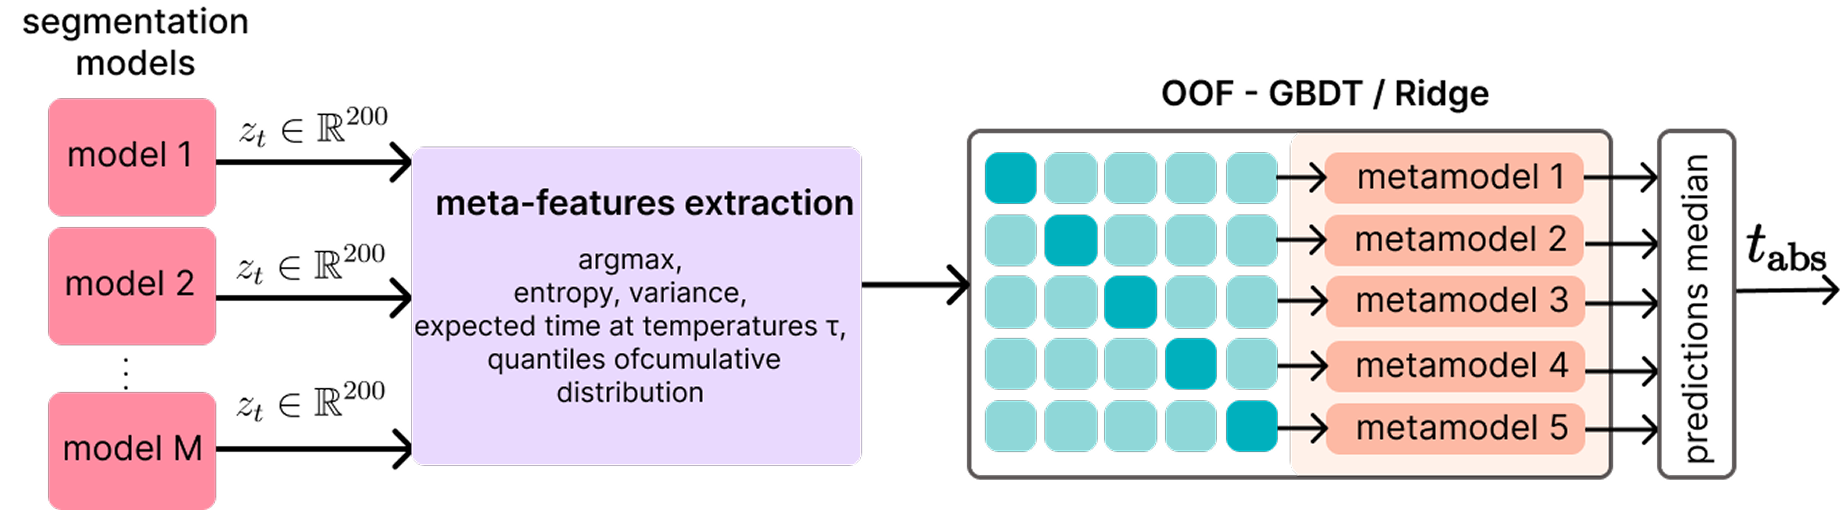
\includegraphics[width=0.9\linewidth]{img/ch1/Ch1_stacking.png}
    \caption{OOF stacking for RT prediction from time-distribution outputs. Per-model logits/distributions are converted into
    meta-features (e.g., peak time, entropy/variance, temperature-conditioned expected times, and CDF quantiles) and combined
    by a second-stage stacker (Ridge/GBDT). Predictions from fold-trained stackers are aggregated at inference (median) to produce the final RT estimate.}
    \label{fig:Ch1_stacking}
\end{figure}

\paragraph{Meta-features from logits and temperature-scaled probabilities.}
Meta-features are extracted per model from (i) raw logits and (ii) temperature-scaled probabilities computed for multiple
temperatures $\tau\in\mathcal{T}_{\text{meta}}$. From logits, a hard-peak estimate and confidence proxies are computed:

\begin{equation}
\label{eq:rt_stacking_logit_features}
t^\star = \arg\max_{t} z_t,\qquad
\hat t_{\mathrm{hard}} = t_0 + g_{t^\star},\qquad
z_{\max} = \max_t z_t,\qquad
m_{\mathrm{top2}} = z_{\max} - \max_{t\neq t^\star} z_t.
\end{equation}
For each $\tau\in\mathcal{T}_{\text{meta}}$, probabilities are formed as $p(\tau)=\mathrm{softmax}(\mathbf{z}/\tau)$ (Eq.~\ref{eq:rt_pred_dist}, Sec.~\ref{sec:event_time_formulation}), where $\mathbf{z}=(z_0,\dots,z_{T-1})$ denotes the per-time logit vector for a given model and window. Distributional summaries
are computed, including the soft-argmax time (Eq.~\ref{eq:rt_soft_argmax}, Sec.~\ref{sec:event_time_formulation}), entropy $H(p(\tau))$, peak probability
$p_{\max}(\tau)$, time variance $\mathrm{Var}_{p(\tau)}[g]$, and CDF time-quantiles (10/50/90\%). In our implementation,
$\mathcal{T}_{\text{meta}}=\{0.7,1.0,1.3\}$.

\paragraph{Meta-learner and inference.}
We use linear Ridge regression as a strong baseline meta-learner, and gradient boosting to capture non-linear reliability
patterns across models and temperatures. The meta-learner is trained using subject-disjoint cross-validation: each subject is assigned to exactly one fold (Figure~\ref{fig:Ch1_stacking}). For fold $k$, the stacker is fit on the other folds and predicts RT for the held-out fold. The leakage-controlled diagnostic is the out-of-fold nRMSE from these held-out predictions. Folds are stratified to match the per-subject mean RT distribution across folds. For held-out inference, the same feature construction is applied to unseen logits; predictions from the fold-trained stackers are aggregated to obtain the final RT estimate.
Manual blending serves as a reference, but it cannot adapt weights to sample-specific confidence profiles.

\section{Original Hidden CodaBench Benchmark Results}

We report the original hidden-release CodaBench evaluation as historical challenge context. These scores provide continuity with the original benchmark setting, while the main empirical conclusions in this manuscript are based on the labeled R11 release with subject-bootstrap confidence intervals.

\begin{table}[!h]
\centering
\caption{Original hidden-release CodaBench RT results from the earlier submission-oriented pipeline. These results are reported for historical comparison with the challenge setting.}
\label{tab:appendix_codabench}
\small
\setlength{\tabcolsep}{8pt}
\renewcommand{\arraystretch}{1.15}
\begin{tabular}{lcc}
\toprule
\textbf{Method} & \textbf{Validation nRMSE} $\downarrow$ & \textbf{Hidden nRMSE} $\downarrow$ \\
\midrule
Best temperature-tuned single model & 0.898757 & 0.92334 \\
Manual blending & 0.899979 & 0.91840 \\
Ridge stacking & 0.890430 & 0.91539 \\
Gradient boosting stacking & \textbf{0.883365} & \textbf{0.91394} \\
\bottomrule
\end{tabular}
\end{table}

\section{Unwrapped External Backbone Sanity Checks}

Unwrapped external architectures are useful for diagnosing scale sensitivity. Because our own models use per-window standardization, the primary comparison uses wrapped external models. Table~\ref{tab:appendix_unwrapped_external} reports matched sanity checks for representative off-the-shelf architectures with and without the fixed per-window standardization wrapper. The unwrapped rows often collapse toward target-standard-deviation behavior (nRMSE near 1), whereas the wrapped variants train meaningfully under the same release-separated protocol used in the main tables.

\begin{table}[!t]
\centering
\caption{Unwrapped external-backbone sanity checks. ``Wrapped'' means that the model receives the same per-window channel standardization used by our compact baselines. These checks diagnose scale sensitivity; the wrapped variants are the fair external comparisons used in the main results.}
\label{tab:appendix_unwrapped_external}
\scriptsize
\setlength{\tabcolsep}{3pt}
\renewcommand{\arraystretch}{1.12}
\resizebox{\linewidth}{!}{%
\begin{tabular}{@{} l c c c c l @{}}
\toprule
\textbf{Architecture} & \textbf{Unwrapped valid} & \textbf{Unwrapped R11} & \textbf{Wrapped valid} & \textbf{Wrapped R11} & \textbf{Takeaway} \\
\midrule
EEGNet & 1.000000 & 1.002046 [0.999718, 1.007253] & 0.957877 & 0.965041 [0.954684, 0.977111] & Standardization makes the compact EEG baseline train \\
EEGConformer & 1.000000 & 1.000413 [0.999906, 1.003179] & 0.957968 & 0.962802 [0.951634, 0.975382] & Transformer-style baseline is scale-sensitive without wrapping \\
LaBraM & 1.000000 & 1.000711 [0.998638, 1.004512] & 0.958254 & 0.965382 [0.952576, 0.979330] & From-scratch foundation-style architecture needs the fixed normalization \\
\bottomrule
\end{tabular}%
}
\end{table}

\section{Additional Protocol Calibration Runs}

Protocol calibration evaluated optimizer choice, learning rate, soft-label width, batch size, and augmentation strength before fixing the training recipe used in the release-separated experiments. These diagnostics informed the protocol but are separated from the R11 results used for the main claims.

\section{Additional EventNLL Kernel and Hazard Robustness Checks}

The main text keeps the event-time segmentation table focused on the core CE, EventNLL, and control objectives, plus two compact EventNLL-family extensions. Table~\ref{tab:appendix_kernel_hazard_robustness} reports the broader kernel and hazard robustness checks. These runs use the same release-separated protocol and test whether the probabilistic event-time result depends on one specific Gaussian observation kernel or one specific softmax parameterization.

\begin{table}[!t]
\centering
\caption{Additional EventNLL kernel and hazard robustness checks. ``Cal.'' denotes post-hoc temperature selection on R9--R10; the heteroscedastic run is reported at its base readout because it was not part of the calibrated kernel table.}
\label{tab:appendix_kernel_hazard_robustness}
\scriptsize
\setlength{\tabcolsep}{3pt}
\renewcommand{\arraystretch}{1.12}
\resizebox{\linewidth}{!}{%
\begin{tabular}{@{} l l c c c l @{}}
\toprule
\textbf{Variant} & \textbf{Change tested} & $\boldsymbol{\tau}$ & \textbf{Valid nRMSE} $\downarrow$ & \textbf{R11 nRMSE} $\downarrow$ & \textbf{Takeaway} \\
\midrule
Gaussian EventNLL, cal. & fixed Gaussian observation kernel & 0.70 & 0.923619 & 0.940947 [0.923160, 0.960322] & Core latent event-time likelihood reference \\
Gaussian mixture EventNLL, cal. & narrow/wide Gaussian observation mixture & 0.75 & 0.921676 & 0.939267 [0.921864, 0.958291] & Strongest calibrated EventNLL-family scalar readout \\
Laplace EventNLL, cal. & Laplace observation kernel & 0.75 & 0.926636 & 0.940696 [0.923718, 0.959285] & Robust kernel did not improve over cleaner Gaussian/mixture variants \\
Student-$t$ EventNLL, cal. & heavy-tailed Student-$t$ observation kernel & 0.80 & 0.923259 & 0.941127 [0.923382, 0.960687] & Calibration recovers validation gap, but R11 remains tied or weaker \\
Heteroscedastic EventNLL & trial-wise learned observation scale $\sigma(x)$ & 0.65 & 0.923056 & 0.942343 [0.923630, 0.962703] & Learned scale did not improve R11 enough for the core table \\
Hazard EventNLL & hazard posterior with continuous Gaussian EventNLL & 0.65 & 0.924318 & 0.937332 [0.920594, 0.955704] & Strong alternative posterior parameterization \\
Hazard discrete NLL & exact-bin discrete survival likelihood & 0.65 & 0.926288 & 0.946823 [0.928204, 0.967220] & Negative control: exact-bin survival loss is weaker than continuous EventNLL \\
\bottomrule
\end{tabular}%
}
\end{table}

Overall, these checks support two points. First, the EventNLL view is not tied to a single Gaussian-softmax implementation: the hazard EventNLL and Gaussian-mixture kernel remain competitive. Second, more robust or more flexible observation models are not automatically better; Laplace, Student-$t$, heteroscedastic, and exact-bin hazard variants are useful robustness probes but do not strengthen the core R11 story enough to feature in the main table.

\section{Additional Architecture Ablations}

Architecture ablations separate formulation effects from capacity and backbone-specific effects. In particular, ETS-U-Net capacity variants, attention bottlenecks, factorized channel interactions, recurrent variants, and EEG-Inception-style segmentation provide complementary checks on whether the event-time formulation depends on a single encoder-decoder instantiation.

\section{Additional Posterior Geometry Examples}

Table~\ref{tab:posterior_geometry_metrics} reports the quantitative posterior metrics behind Figure~\ref{fig:posterior_geometry_main}, and Figure~\ref{fig:posterior_raster_main} shows the corresponding trial-sorted posterior maps in the main text. Figure~\ref{fig:appendix_temperature_sensitivity} shows the development-split temperature curves used to choose post-hoc readout temperatures.

\begin{figure}[!t]
    \centering
    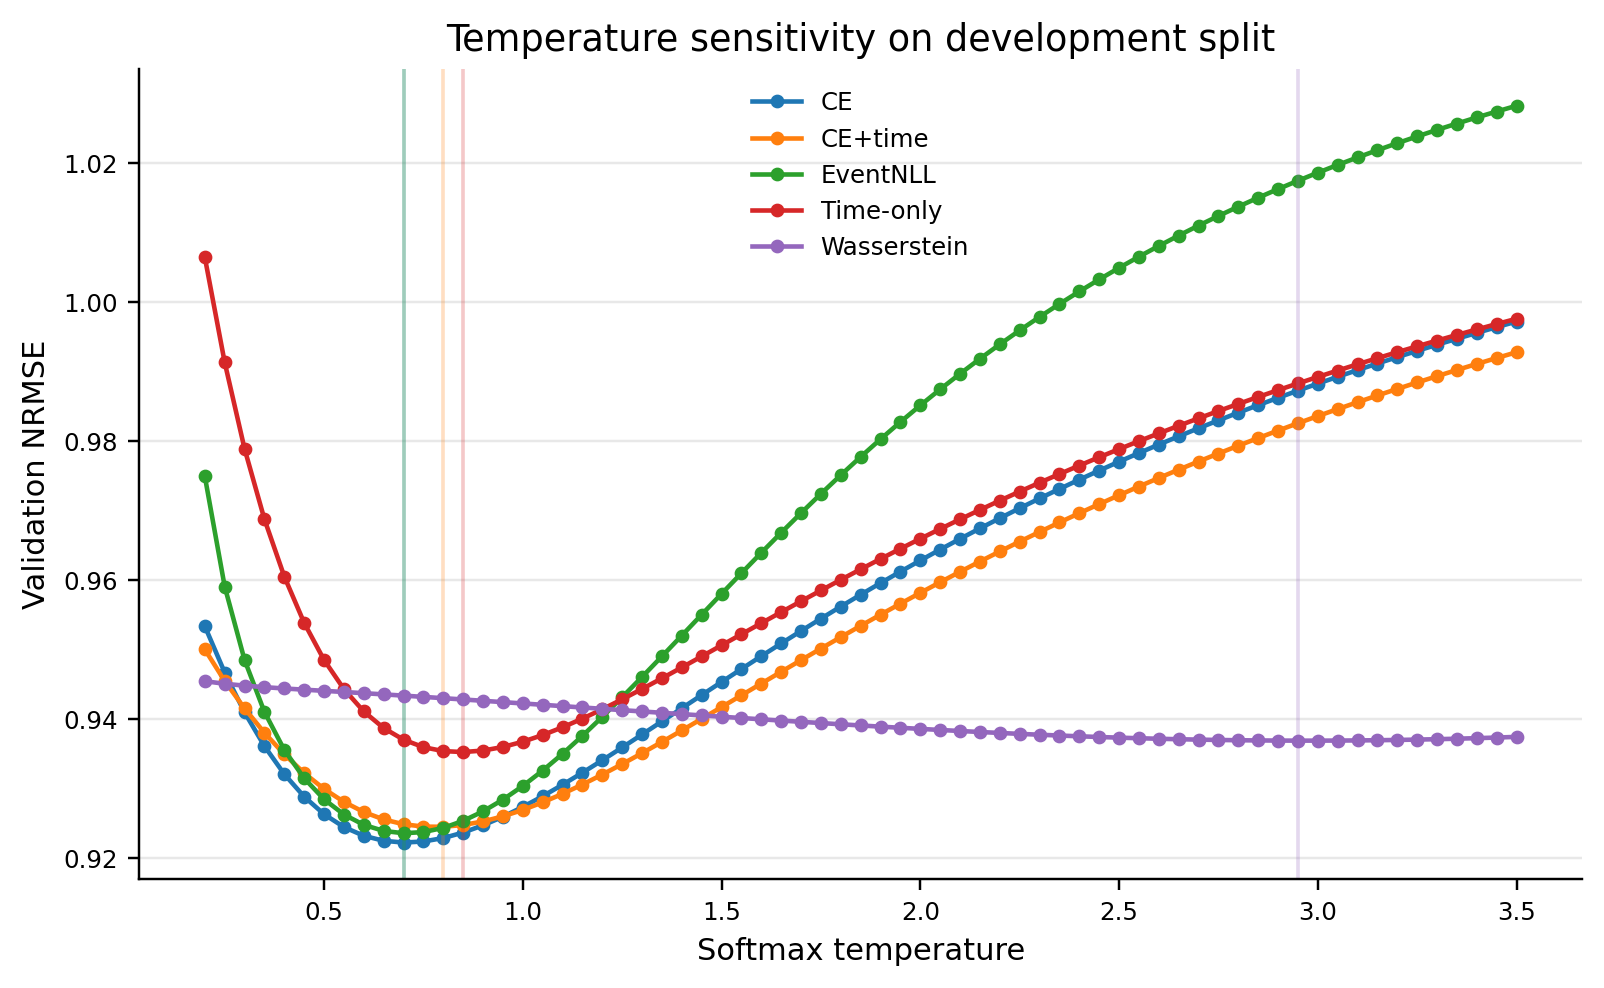
\includegraphics[width=0.9\linewidth]{img/ch1/temperature_sensitivity_calibrated.png}
    \caption{Temperature sensitivity on the R9-R10 development split. Vertical lines mark selected temperatures. The curves show that different losses induce different confidence scales, motivating temperature calibration as posterior-geometry control before comparing scalar readouts or using posterior features downstream.}
    \label{fig:appendix_temperature_sensitivity}
\end{figure}


\FloatBarrier
\clearpage
\bibliography{../references}






% \bibliographystyle{APA}
% \begin{thebibliography}{100}
% \providecommand{\natexlab}[1]{#1}
% \expandafter\ifx\csname urlstyle\endcsname\relax
%   \providecommand{\doi}[1]{doi:\discretionary{}{}{}#1}\else
%   \providecommand{\doi}{doi:\discretionary{}{}{}\begingroup
%   \urlstyle{rm}\Url}\fi

% \bibitem[{LastName(2009)}]{Ref2009}
% LastName, A. (2009).
% \newblock Title for the first reference.
% \newblock \emph{Journal of the first reference}, \emph{3}, 18 -- 88.


% \bibitem[{Authors et~al.(2008)Author1, Author2, \&
%   Author3}]{Ref2008}
% Author1, A., Author2, A., \& Author3, A. (2008).
% \newblock Title for the second reference.
% \newblock \emph{Journal for the second reference}, \emph{5}, 188 -- 200.

% \end{thebibliography}
\end{document}
